\documentclass[../TinyBot.tex]{subfiles}
\begin{document}

\section{Construction} \label{sec:construction}

The first step is to cut out your base material. This can be any material stiff enough to support the Arduino, breadboard, and motors. The club provides corflute, though other materials such as wood or plastic from milk bottles can be used if desired. The base can be any shape, though ensure it is big enough to fit the breadboard, the Arduino you are using if not using a Nano, and a battery.
It is useful to lay out the components you are using on the base material before cutting. \\

\begin{notebox}
    Get creative with the shape of your robot base! Make it a diamond, some kind of squiggle, any shape that fits the components will do!    
\end{notebox}

Once you have cut out the base, peel the backing paper from the breadboard and stick the breadboard to the base.
\begin{center}
    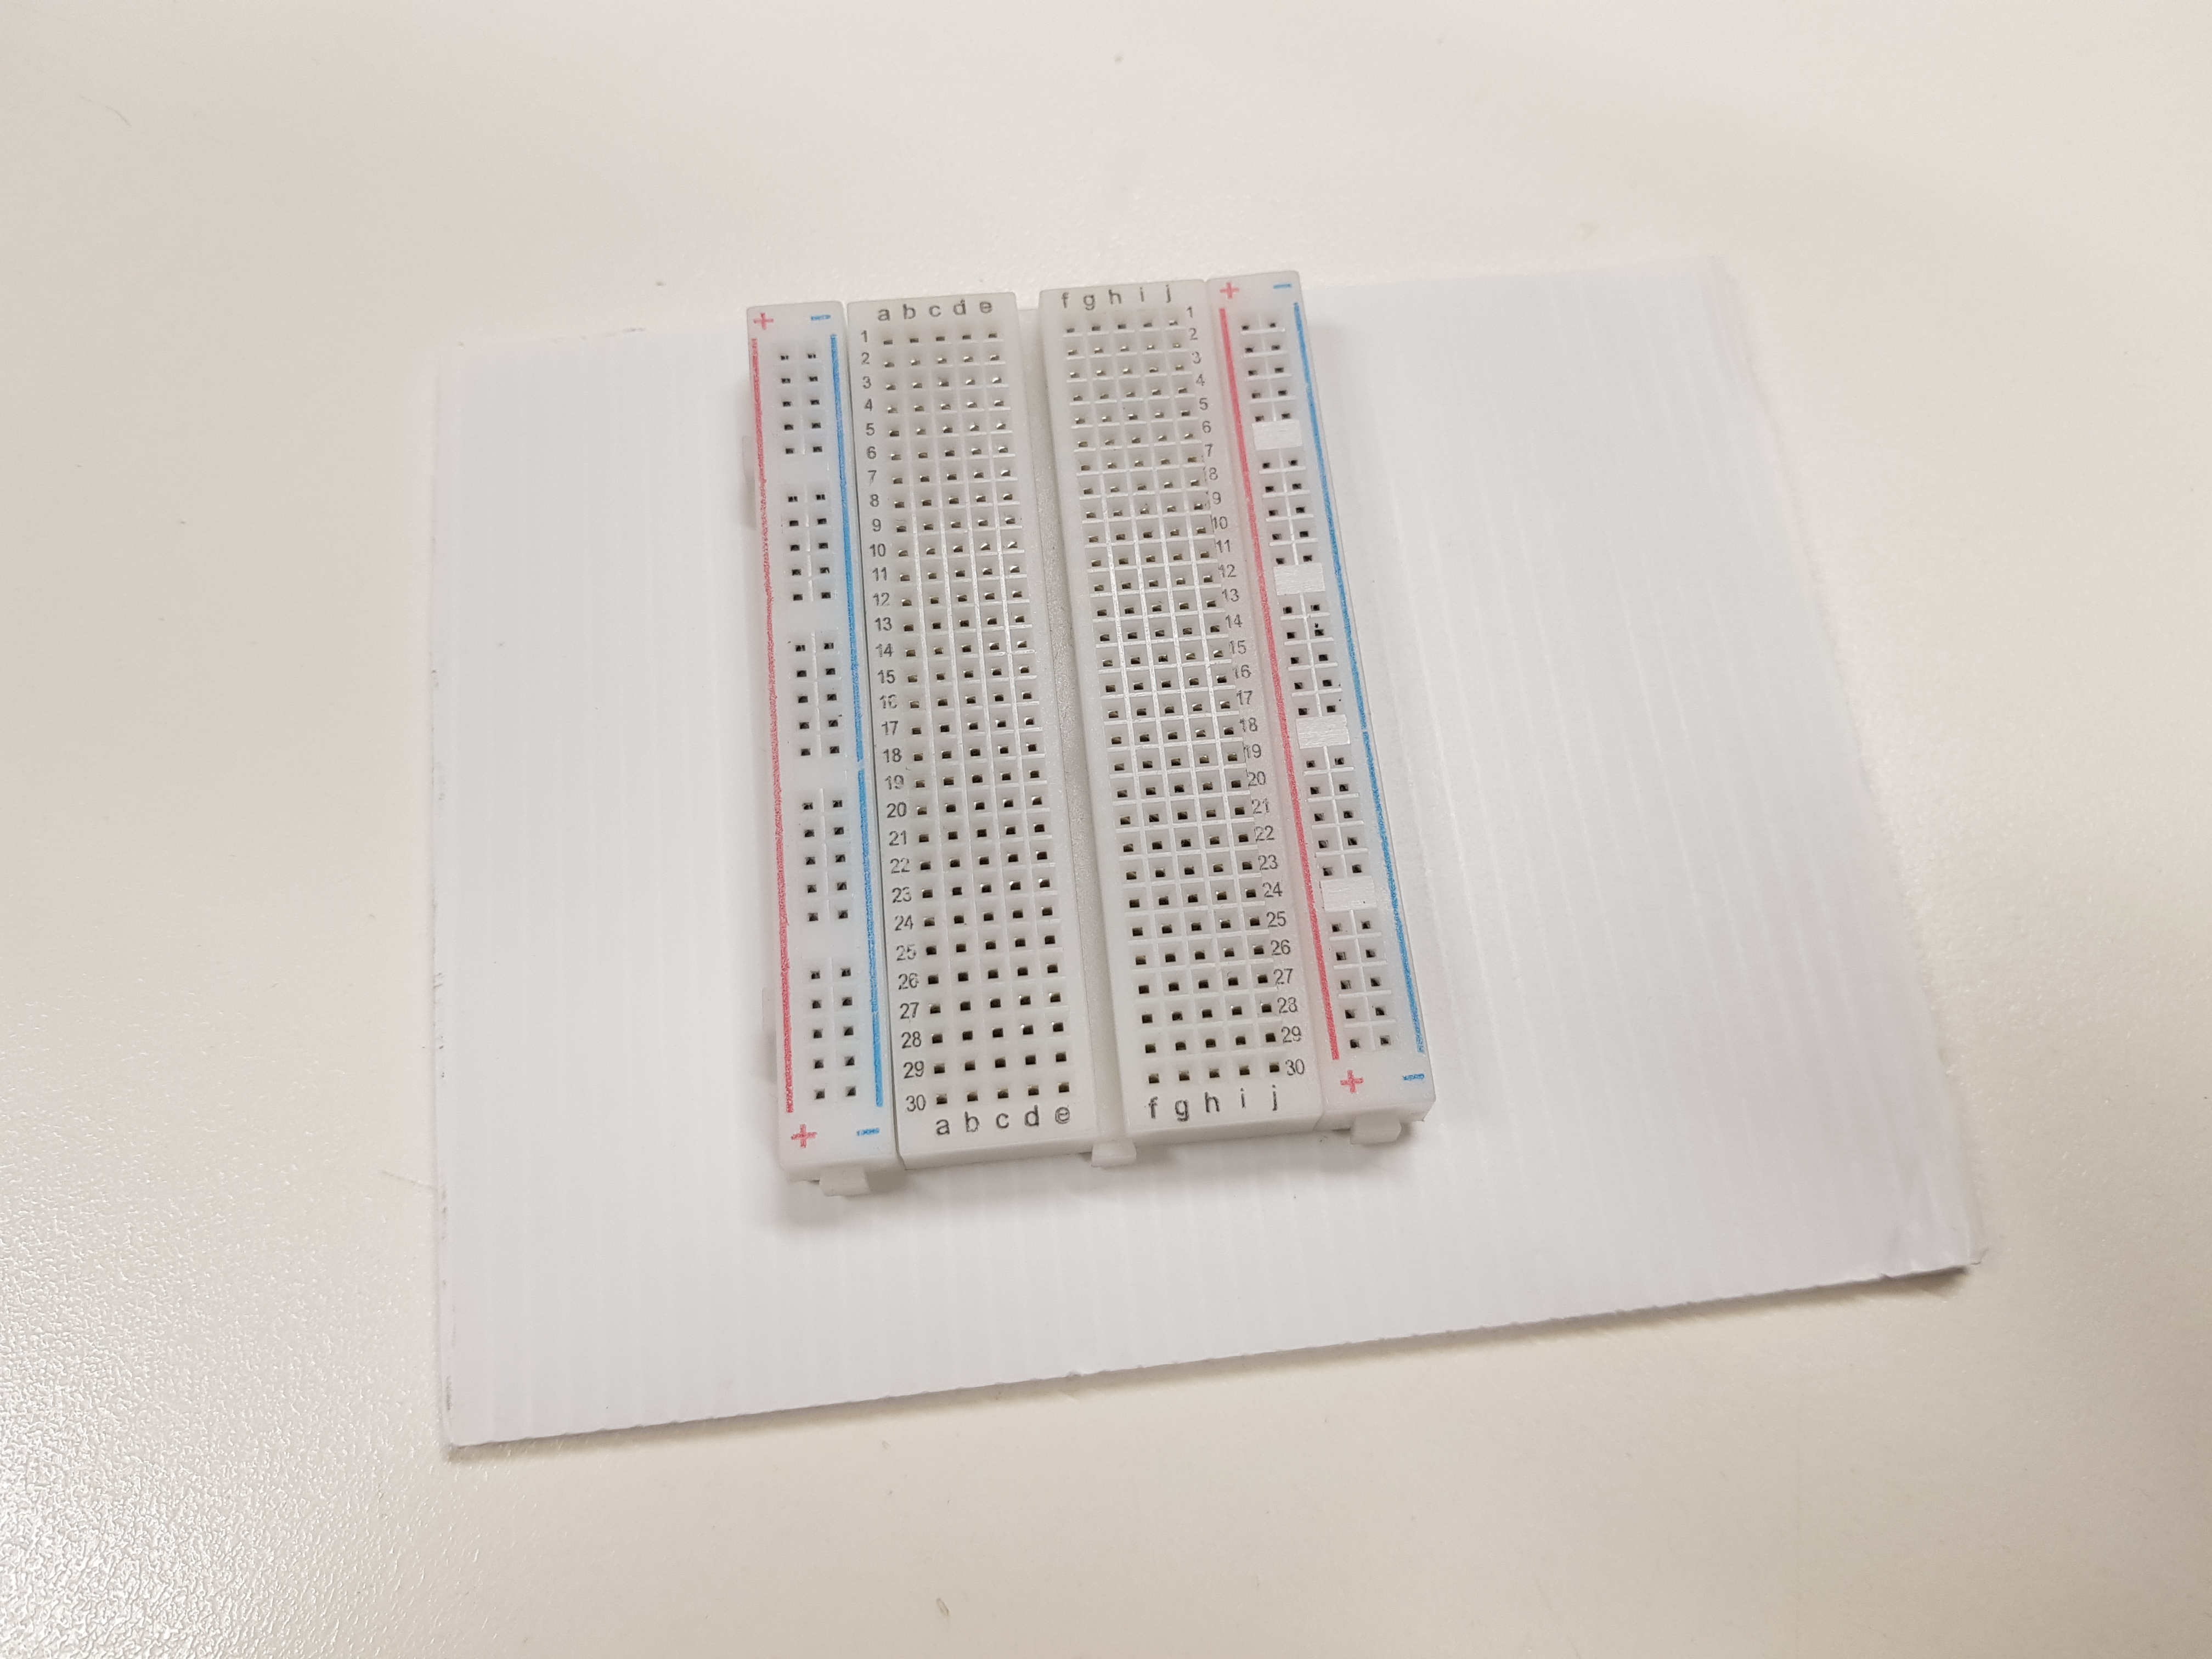
\includegraphics[width=0.6\linewidth]{breadboard_on_base.jpg}
    % \captionof{figure}{fig:construction:breadboard-on-base}
    % \label{fig:construction:breadboard-on-base}
\end{center}

Then place the motor covers and caster wheel on the base and mark out where holes need to be made. The club has plenty of motor covers, though cable ties can be used as an alternative to secure the motors. \\
If using a material like corflute the holes can be marked/made with a screwdriver. Holes will have to be marked and made differently if using other materials. 

\begin{minipage}[t]{0.475\textwidth} \vspace{0pt}
    \begin{center}
        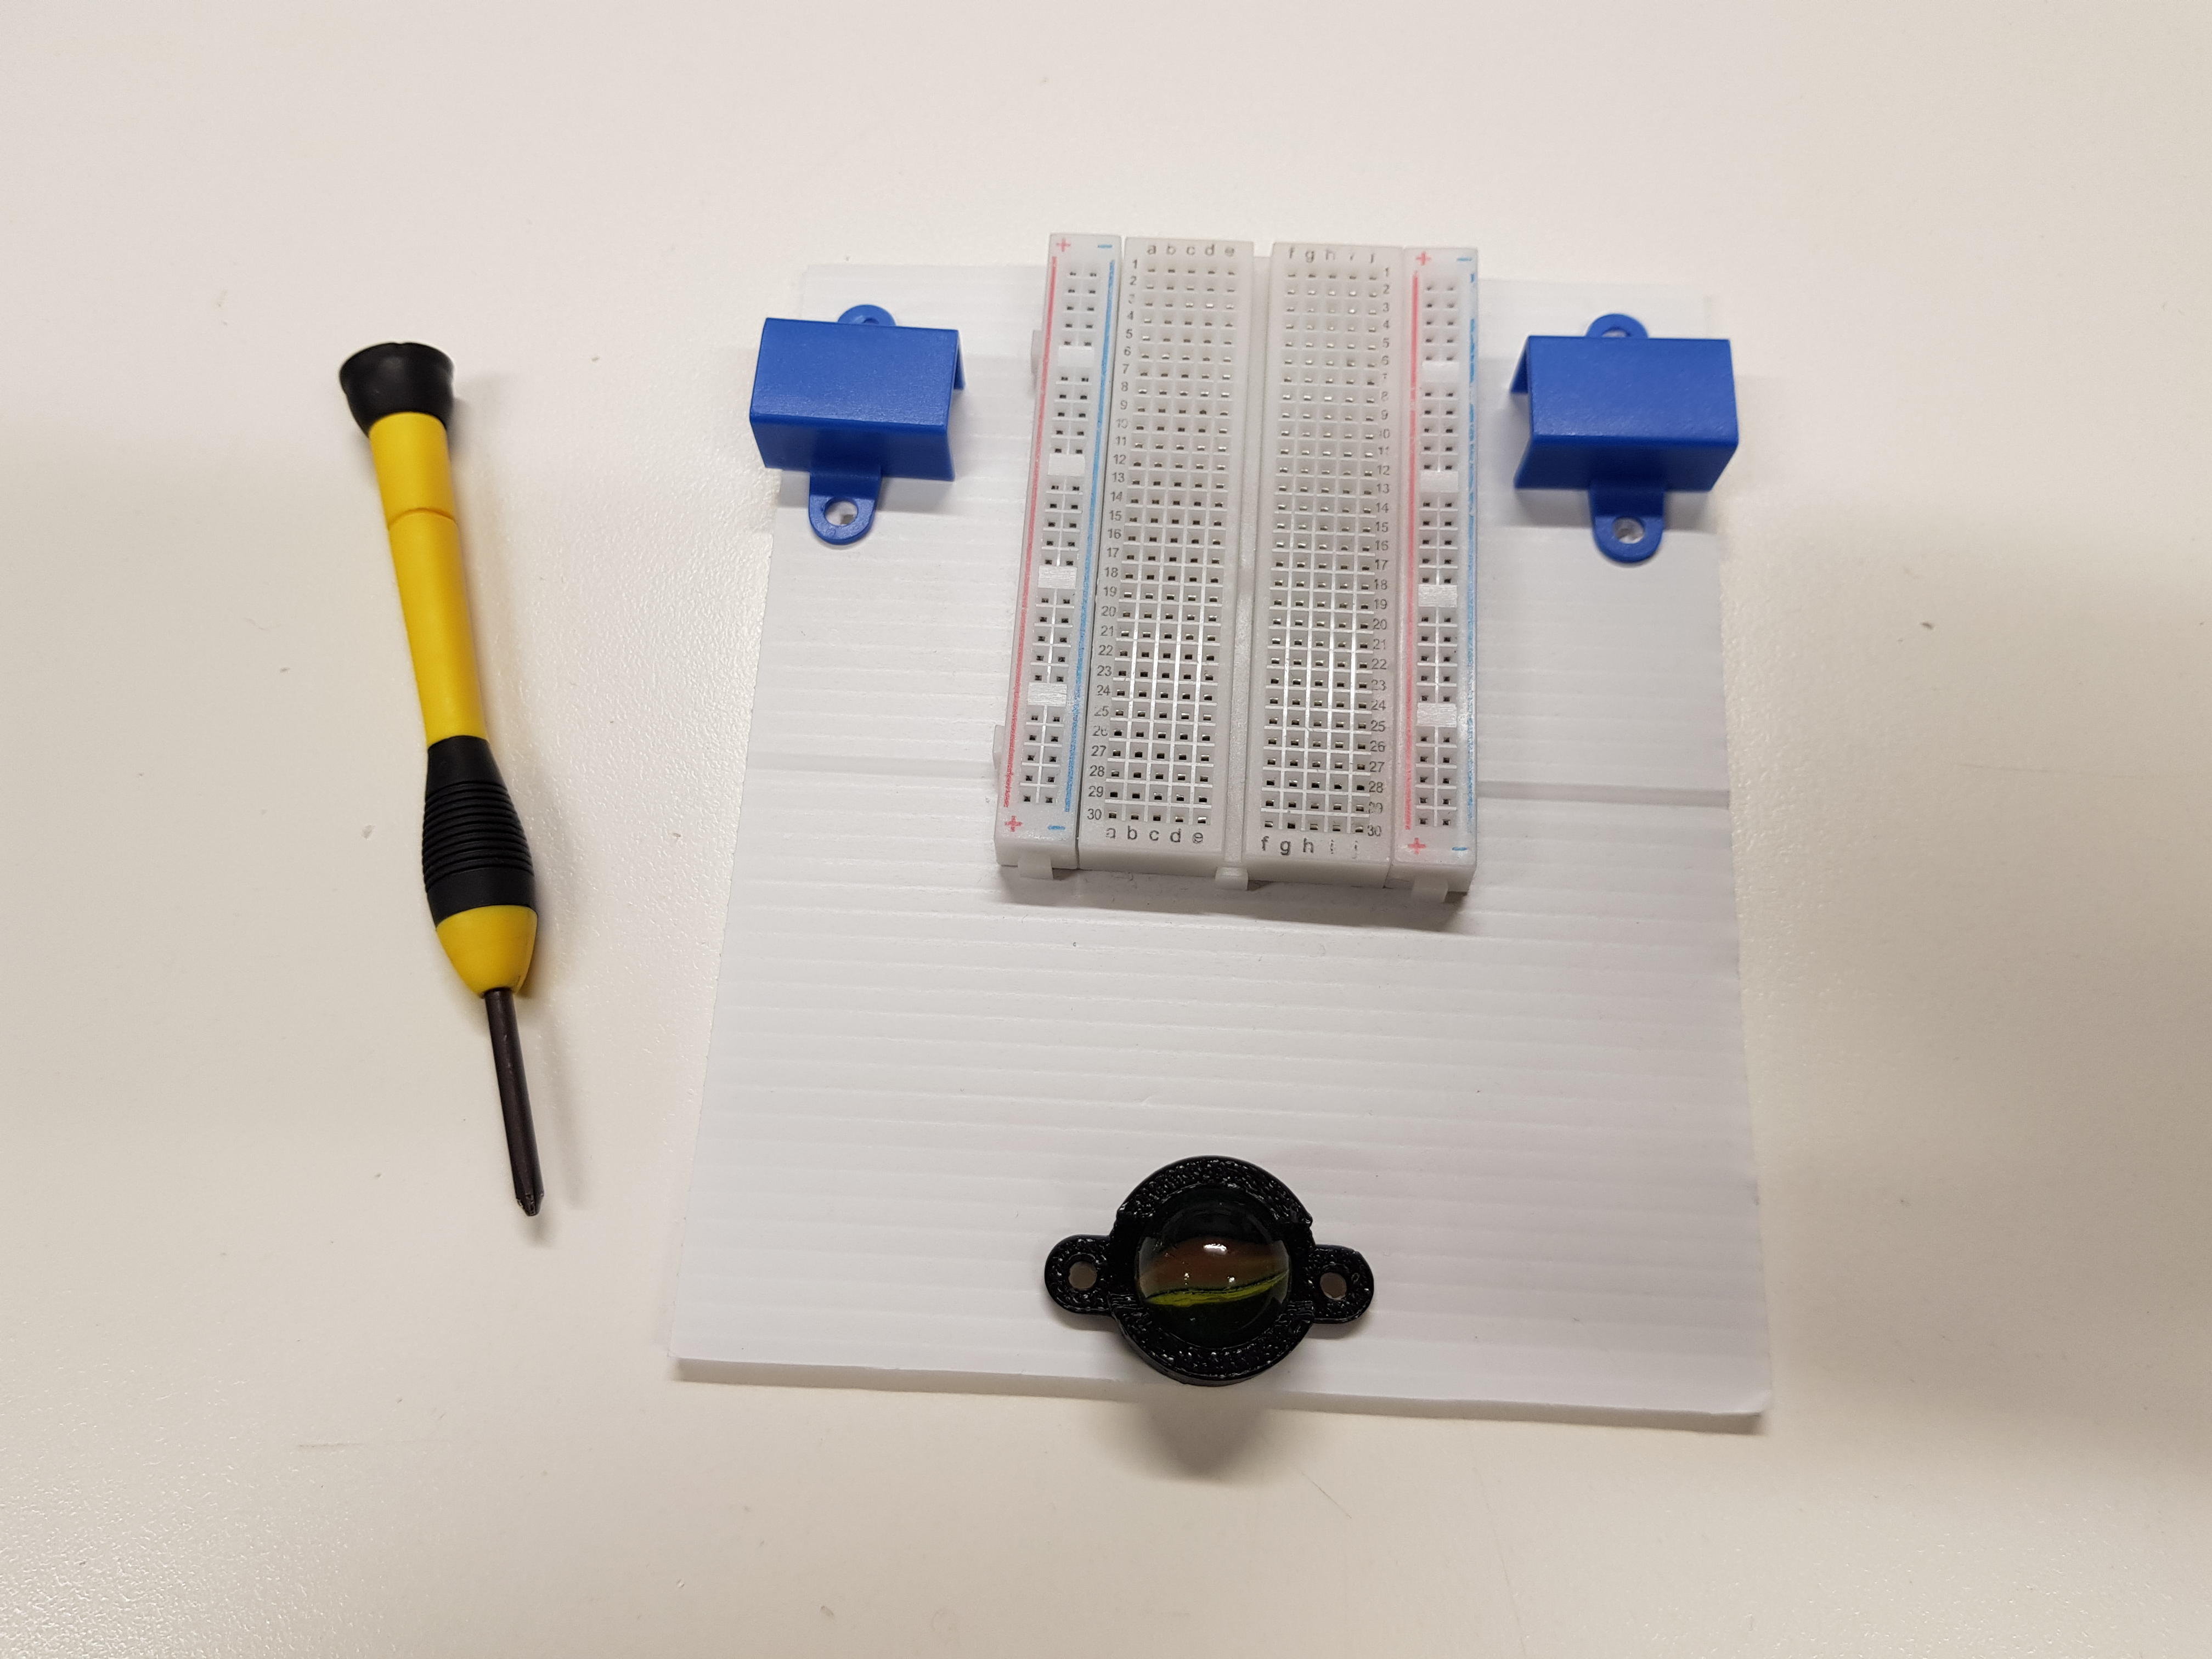
\includegraphics[width=\linewidth]{lining_up_holes_base_screwdriver.jpg}
    \end{center}
\end{minipage}\hfill
\begin{minipage}[t]{0.475\textwidth} \vspace{0pt}
    \begin{center}
        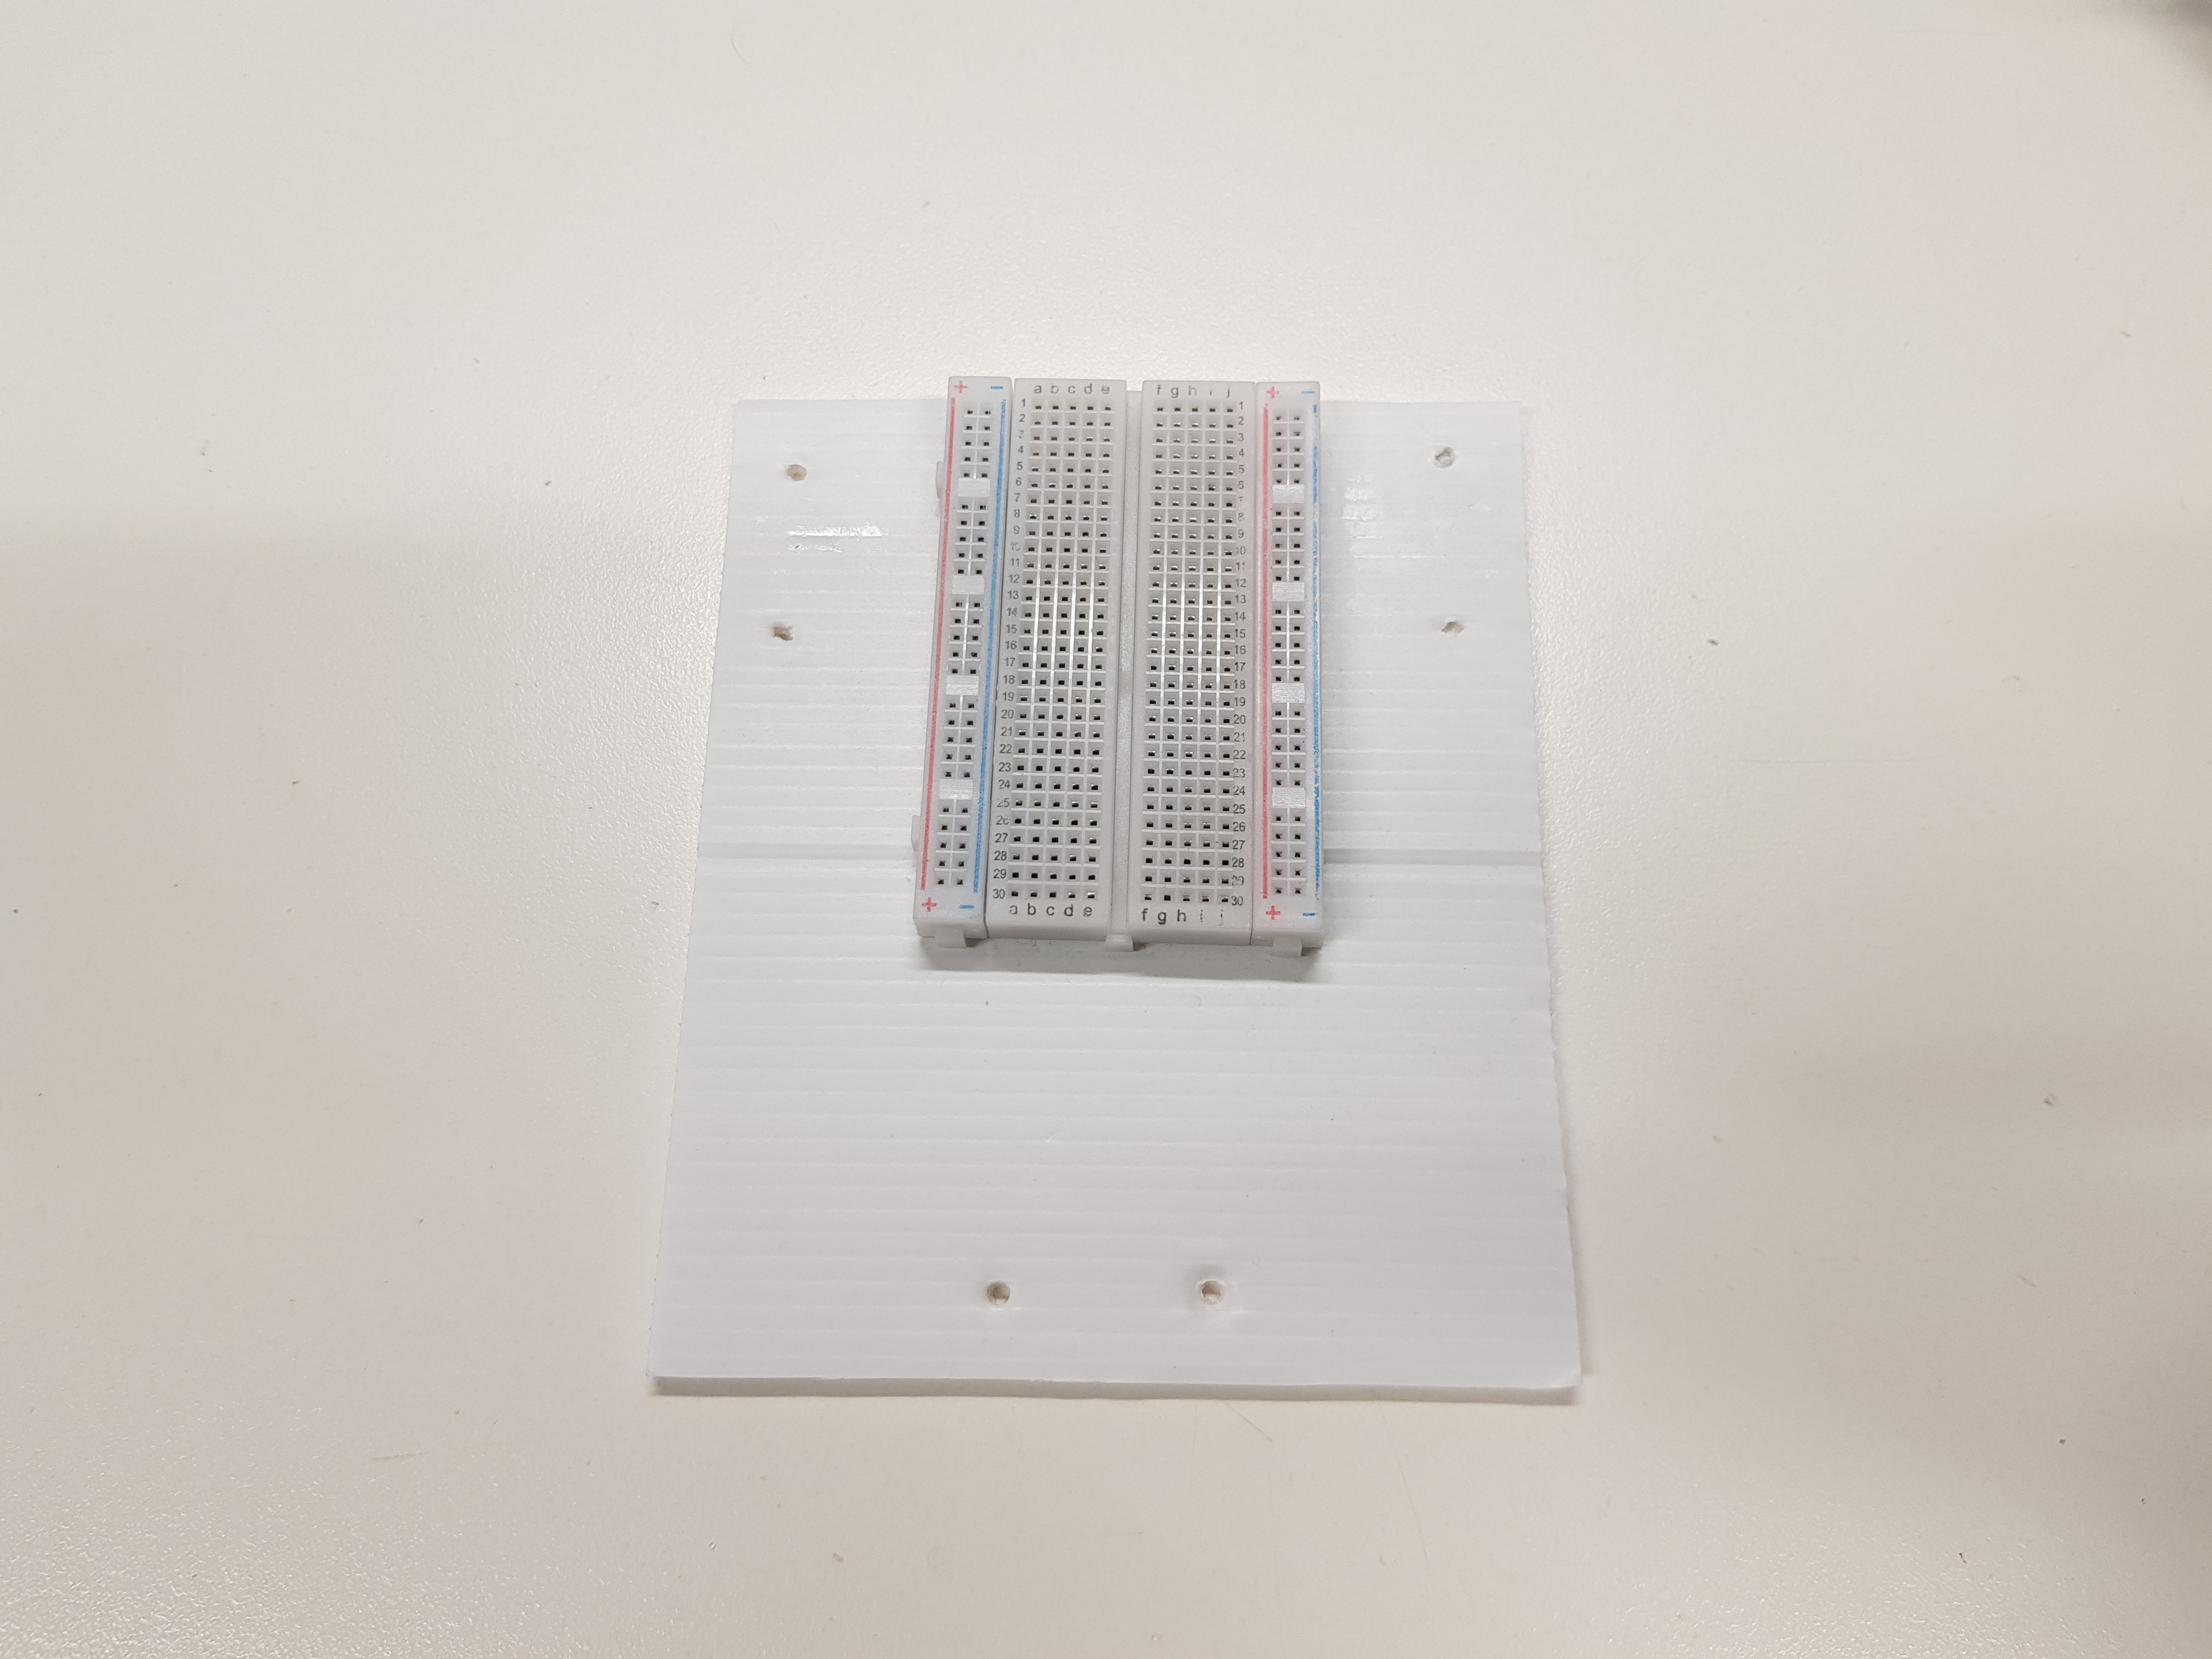
\includegraphics[width=\linewidth]{base_with_holes.jpg}
    \end{center}
\end{minipage}

\bigskip 
It is easier to wire the circuit after the breadboard is stuck to the base as you don't have to worry about pulling any wires out when sticking on the breadboard. The steps to wire up TinyBot are shown below. 
Before starting to wire up the circuit, double check your H-Bridge is in fact a H-Bridge; a lot of IC chips look really similar and are difficult to tell apart. On the back of your chip there should be some serial numbers, make sure that one of these numbers is L293D - there are lots of variations of this H-Bridge so numbers like L293DE are also valid H-Bridges. \\


\begin{center}
    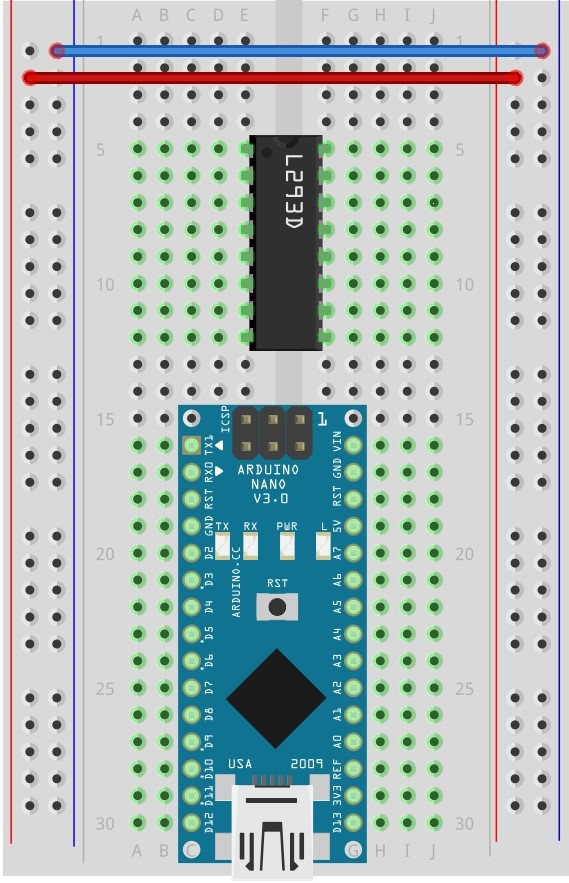
\includegraphics[width=0.3\textwidth]{wiring-step1.jpg}
\end{center}

If you are using an Arduino Nano, push the Nano into the breadboard so that the header pins (the metal "legs") go into the breadboard. Make sure the USB connector is facing out so you can plug the USB cable in later. Also push the H-Bridge in the breadboard, paying attention to where the notch on the IC is. Connect the power and ground rails along each side with a cable. Connecting the rails in this manner allows power and ground to be plugged into either side and still get power. You nearly always want to do this with the ground rail, but sometimes it's useful to have different voltages in the rails on either side and in this case you don't want to connect the power rails. \\
\pagebreak

Next we want to wire up the H-Bridge. This is where the pinout diagram from earlier is very useful. 

\begin{minipage}[t]{0.25\textwidth}\vspace{0pt}
        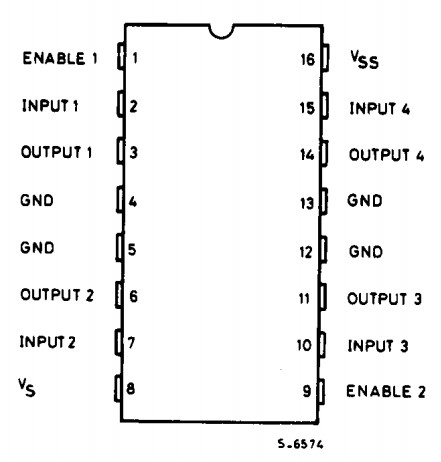
\includegraphics[width=\textwidth]{L293D-pinout.jpg}
\end{minipage} \hfill
\begin{minipage}[t]{0.77\textwidth} \vspace{0pt}
    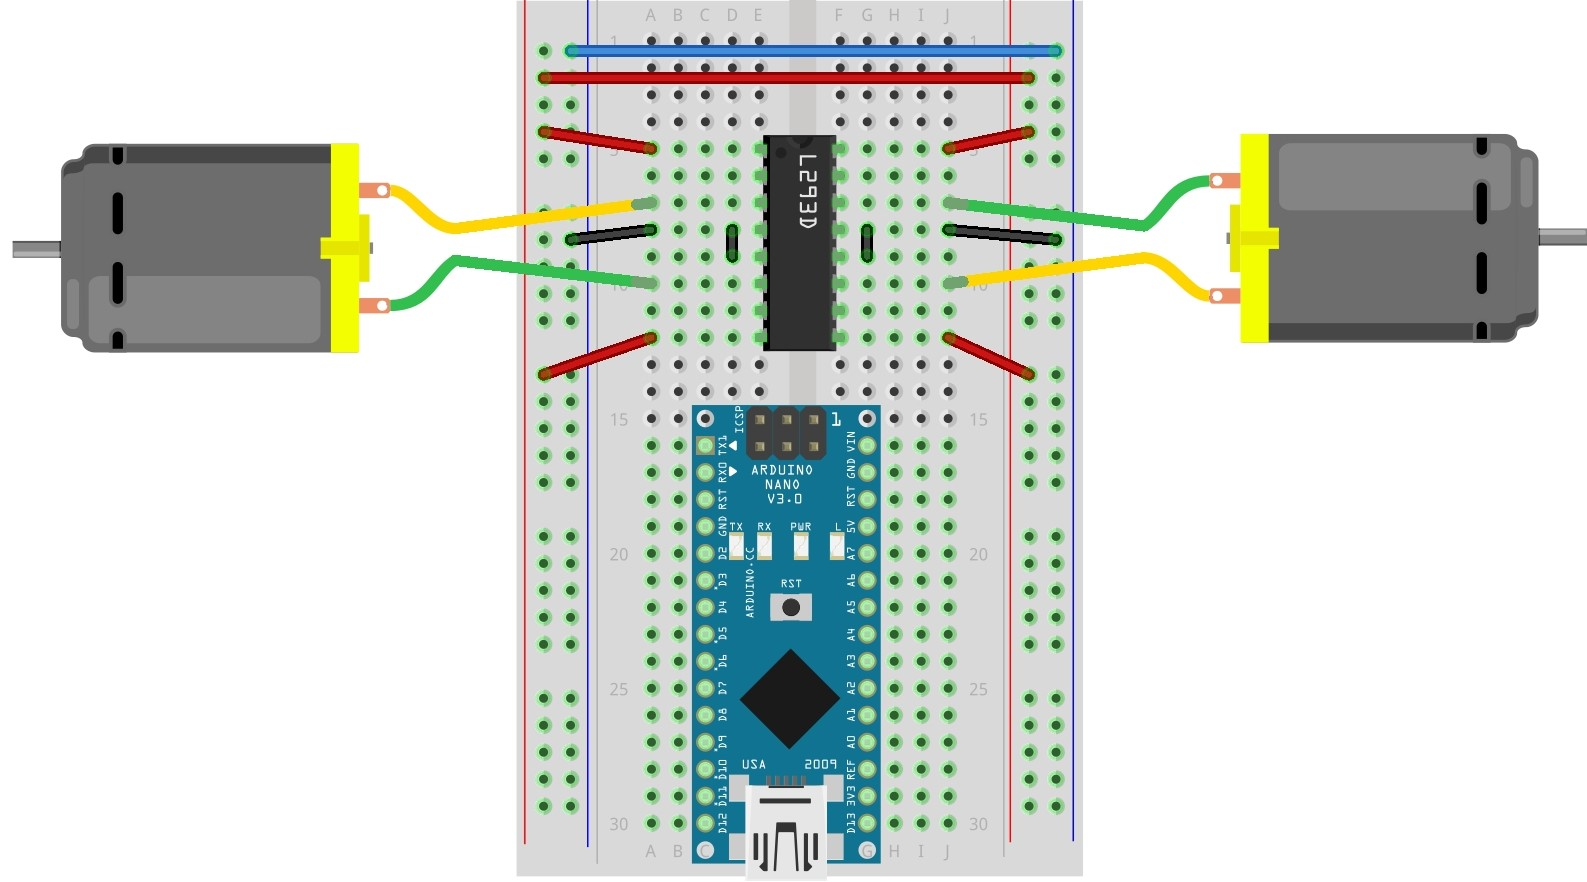
\includegraphics[width=\textwidth]{wiring-step2.jpg}
\end{minipage}
\bigskip

First, connect all the pins labelled ground. Using the pinout, we can see that the four central pins are all GND and so are connected in the wiring diagram. Next, we wire all the enable and $V_S$ pins to the power rail. Then we can connect the motor leads to the output pins. \\

Output pins 1 and 2 are for one motor, and output pins 3 and 4 are for the second motor. Which lead gets plugged into which output pin doesn't matter too much, if you get the pins wrong, nothing will break - the motor will just spin backwards. If you need to swap the motor direction later, just swap the green and yellow leads around. 

\bigskip



% Make sure to check which wire is the positive wire on the motor you have, it should be written on the back plate of the motor. Plugging the motor in backwards will not break anything, the motor will just spin backwards. 

% Swapping the motor direction can be done by swapping the green and yellow wires attached to the motor. 

\begin{center}
    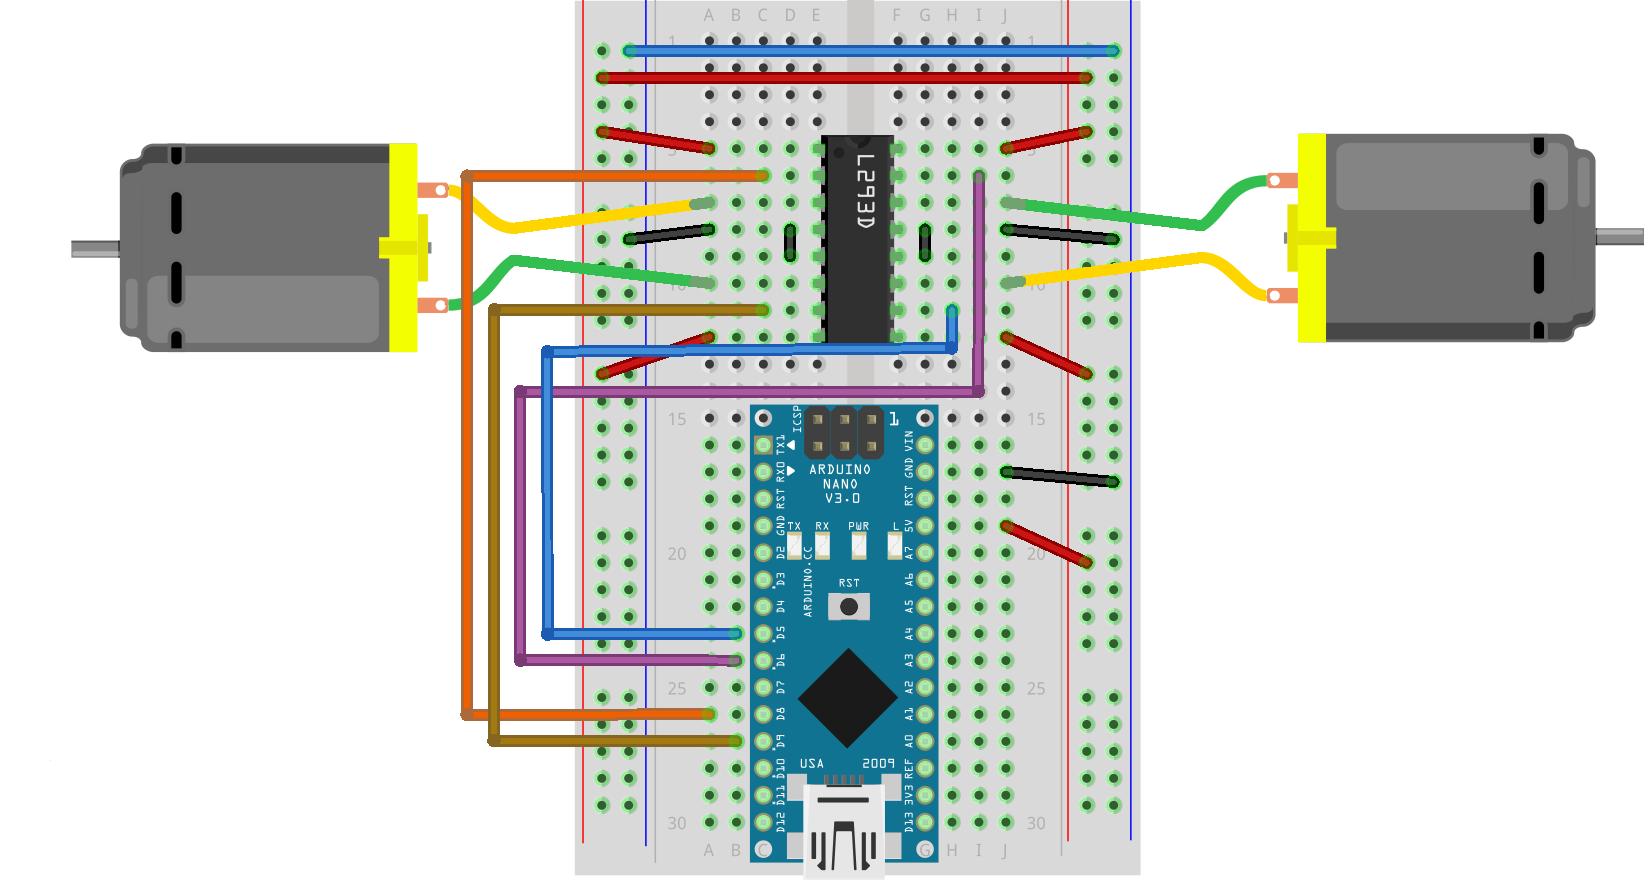
\includegraphics[width=\textwidth]{resources/H-bridge-nano-without-battery_bb.png}
    \captionof{figure}{Wiring Schematic for H-Bridge}
    \label{fig:schematic-hbridge-nobattery}
\end{center}


After wiring up the H-Bridge, we can connect it to the Arduino. We want to connect all the input pins to the Arduino - these are the pins we'll be setting high and low to control the motor direction. 

The pins used in the wiring diagram are:
\begin{itemize}
    \item Input 4 $\rightarrow$ \lstinline[]!D6!
    \item Input 3 $\rightarrow$ \lstinline[]!D5!
    \item Input 2 $\rightarrow$ \lstinline[]!D9!
    \item Input 1 $\rightarrow$ \lstinline[]!D8!
\end{itemize}

\begin{notebox}
    It doesn't matter which pins on the Arduino are connected to the H-Bridge inputs, but the pin numbers must match up in code and wiring. 
\end{notebox}


It's also important to connect power and ground the Arduino. Currently, we're assuming that the Arduino is being powered via USB; and then is supplying power from the \lstinline[]!5V! pin to the breadboard. This is good for testing, but not very useful when we want to put TinyBot on the floor and let it drive around. \\

So, we want to power TinyBot with a battery so it doesn't have to be connected via USB cable. Luckily the circuit with a battery is very similar. The ground wire connected the Arduino to the ground rail can stay where it is. The 5V wire needs to be unplugged, then \lstinline[]!Vin! (meaning voltage in) needs to be connected to the power rail. Also plug the battery into the power rails - with the black wire from the battery going to the ground rail and the red going to the power rail. This circuit is shown in Figure \ref{fig:schematic-hbridge-battery}.

\begin{warningbox}
    Never put supply voltage into the 3.3V or 5V pins; this will break the Arduino. 
\end{warningbox}

% The circuit with a battery is very similar. Instead of powering the Arduino and circuit with the 9V battery you power the Arduino through USB and the circuit from the 5V output pin. See below for a wiring diagram without the battery.

\begin{center}
    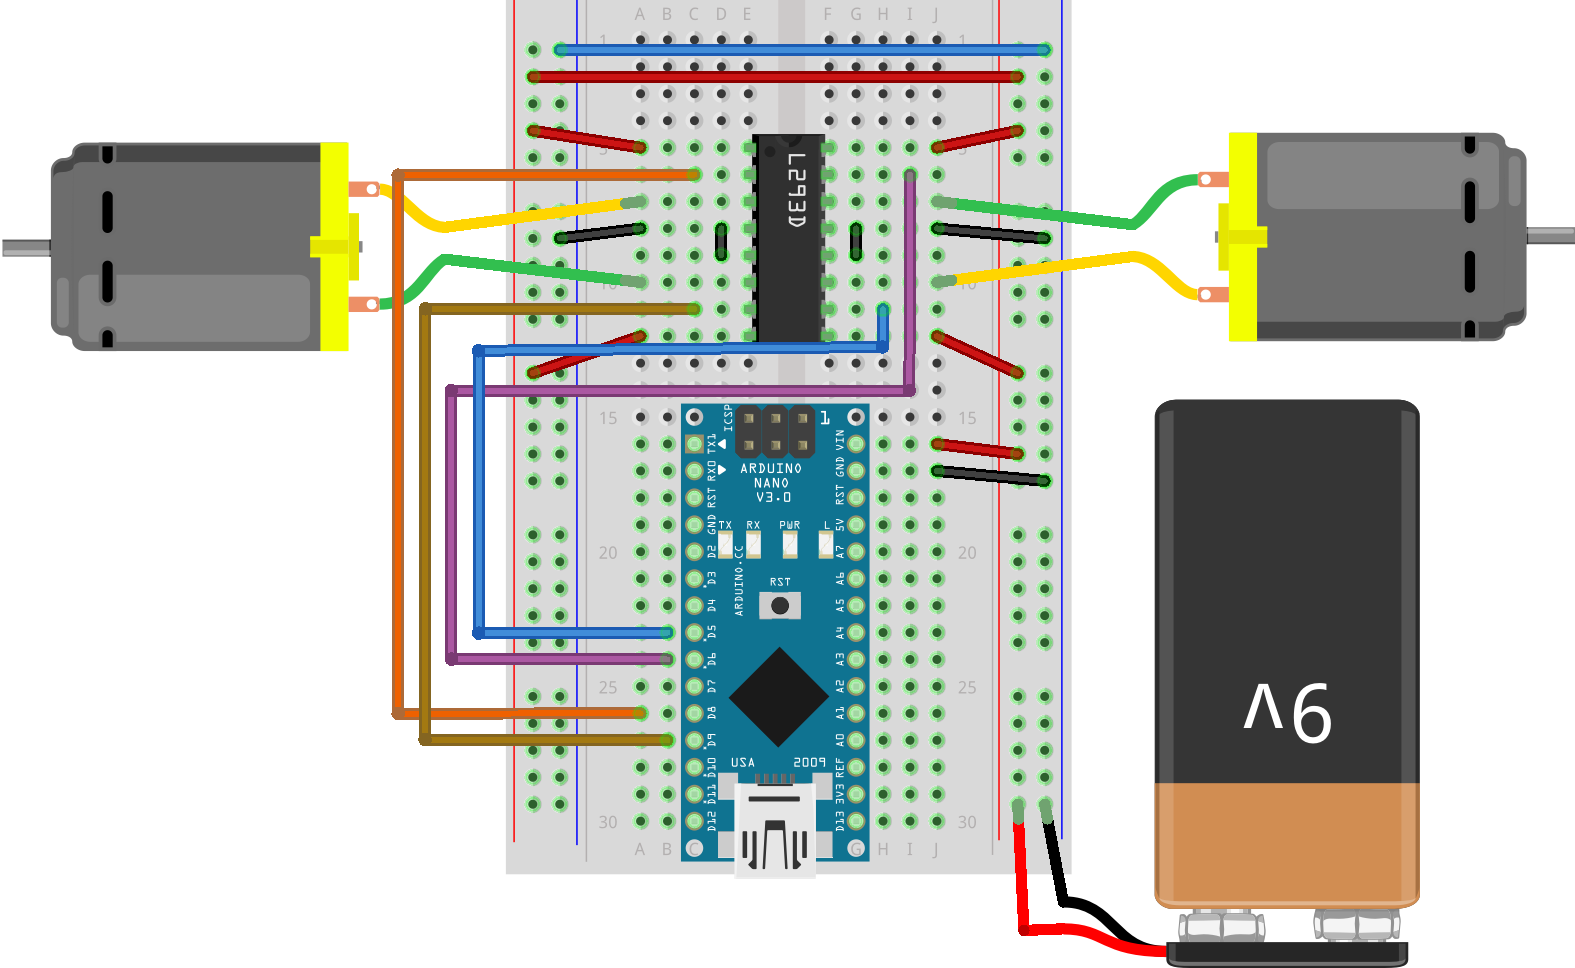
\includegraphics[width=\textwidth]{resources/H-bridge-nano_bb.png}
    \captionof{figure}{Wiring Schematic for H-Bridge}
    \label{fig:schematic-hbridge-battery}
\end{center}



The circuit in real life should look something like this:

\begin{center}
    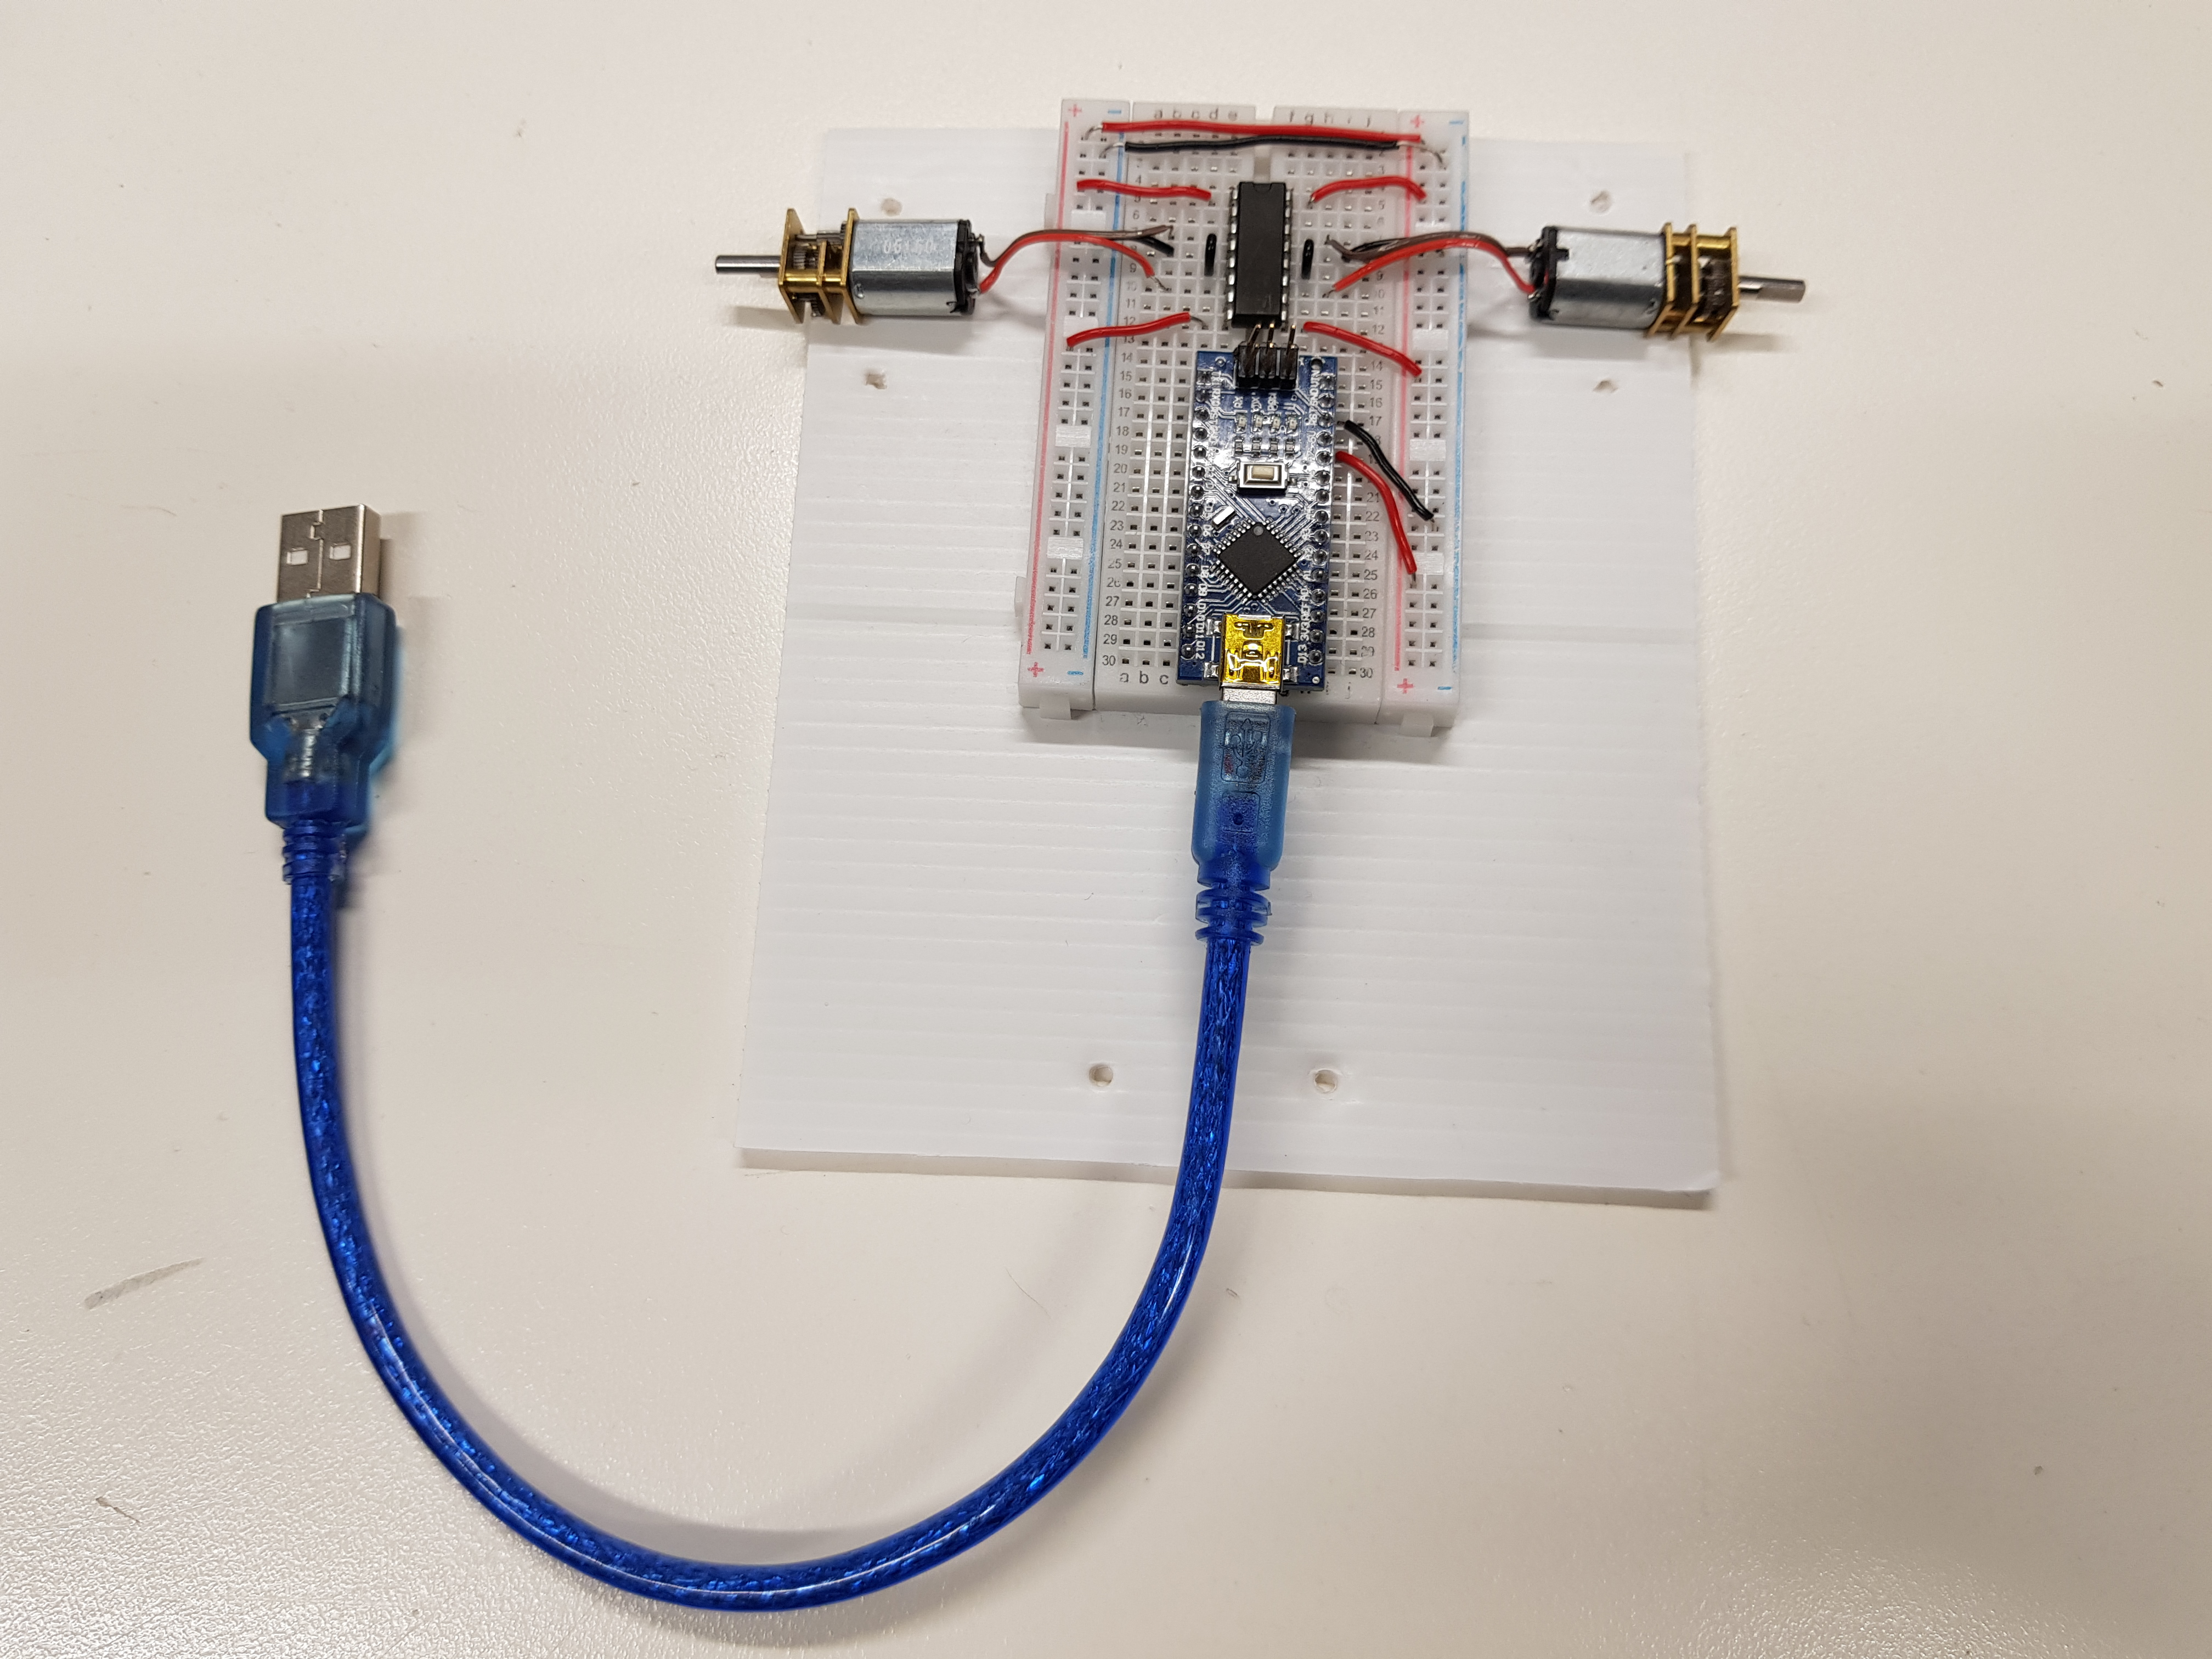
\includegraphics[width=0.6\linewidth]{circuit_on_base.jpg}
\end{center}


% \begin{center}
%     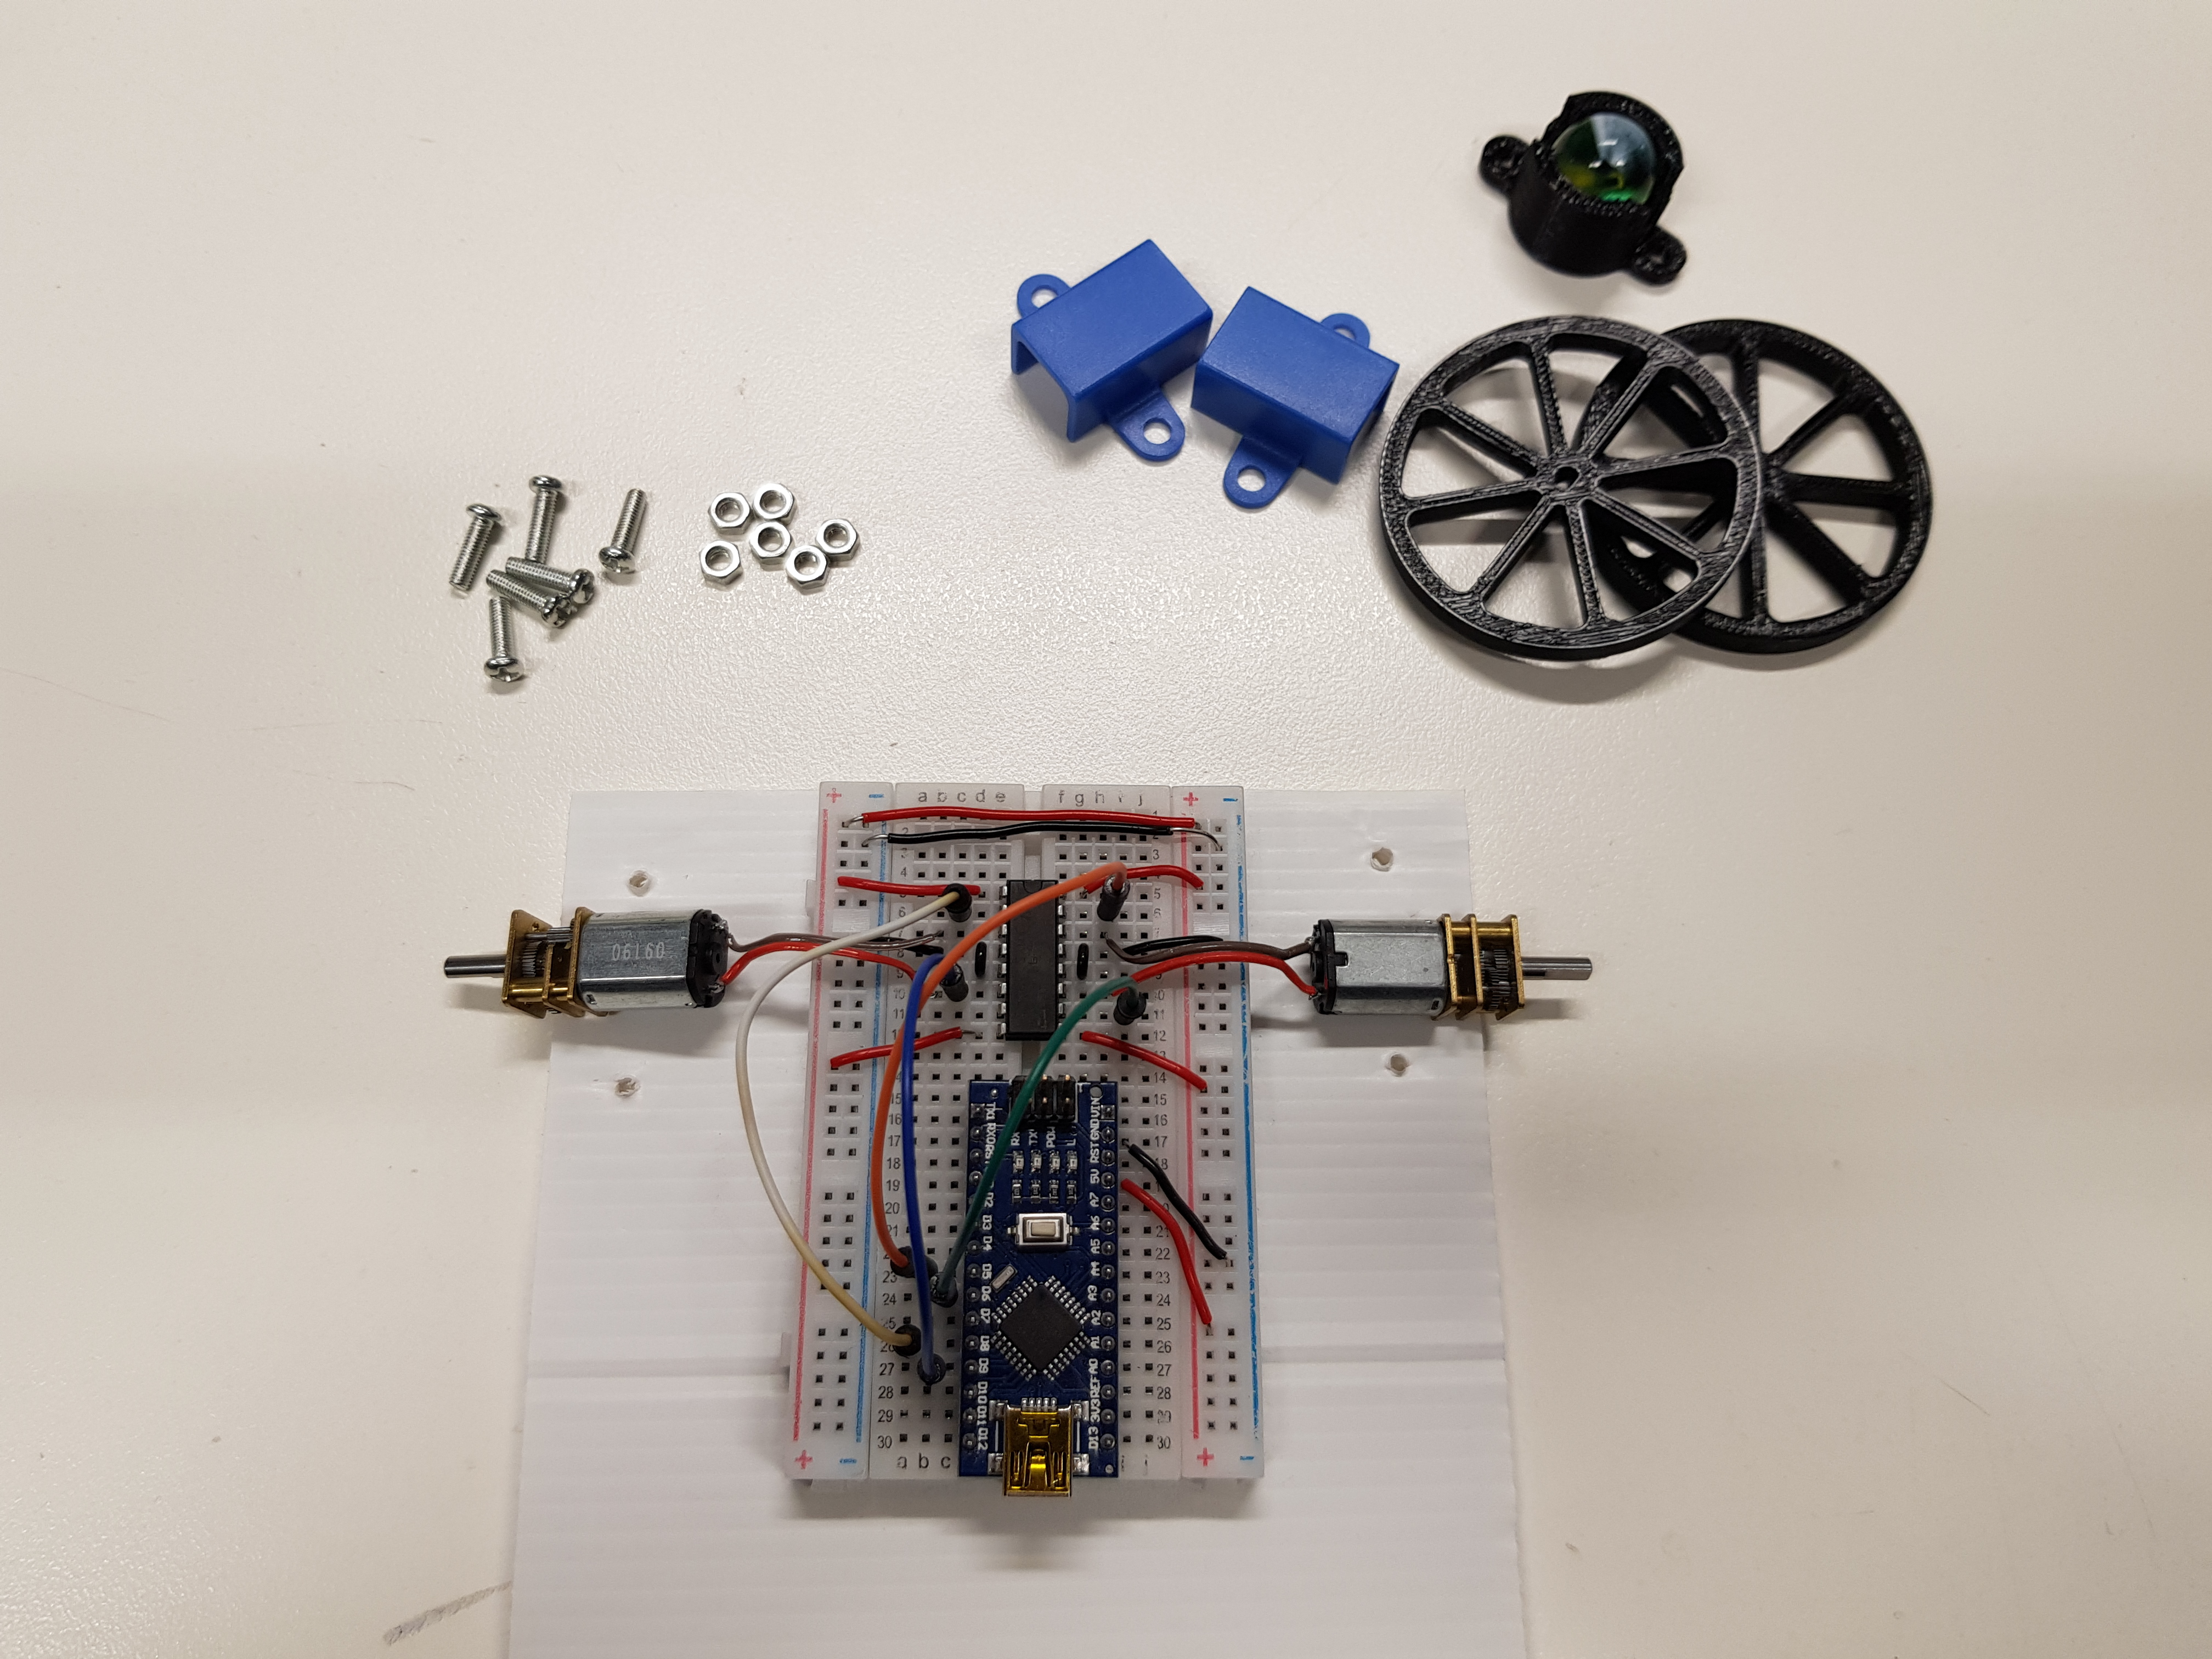
\includegraphics[width=0.6\linewidth]{wired_all_parts.jpg}
% \end{center}
Place the motor covers over the motors and attach to the base using the provided screws. The caster wheel is also attached using screws. 
% \begin{center}
%     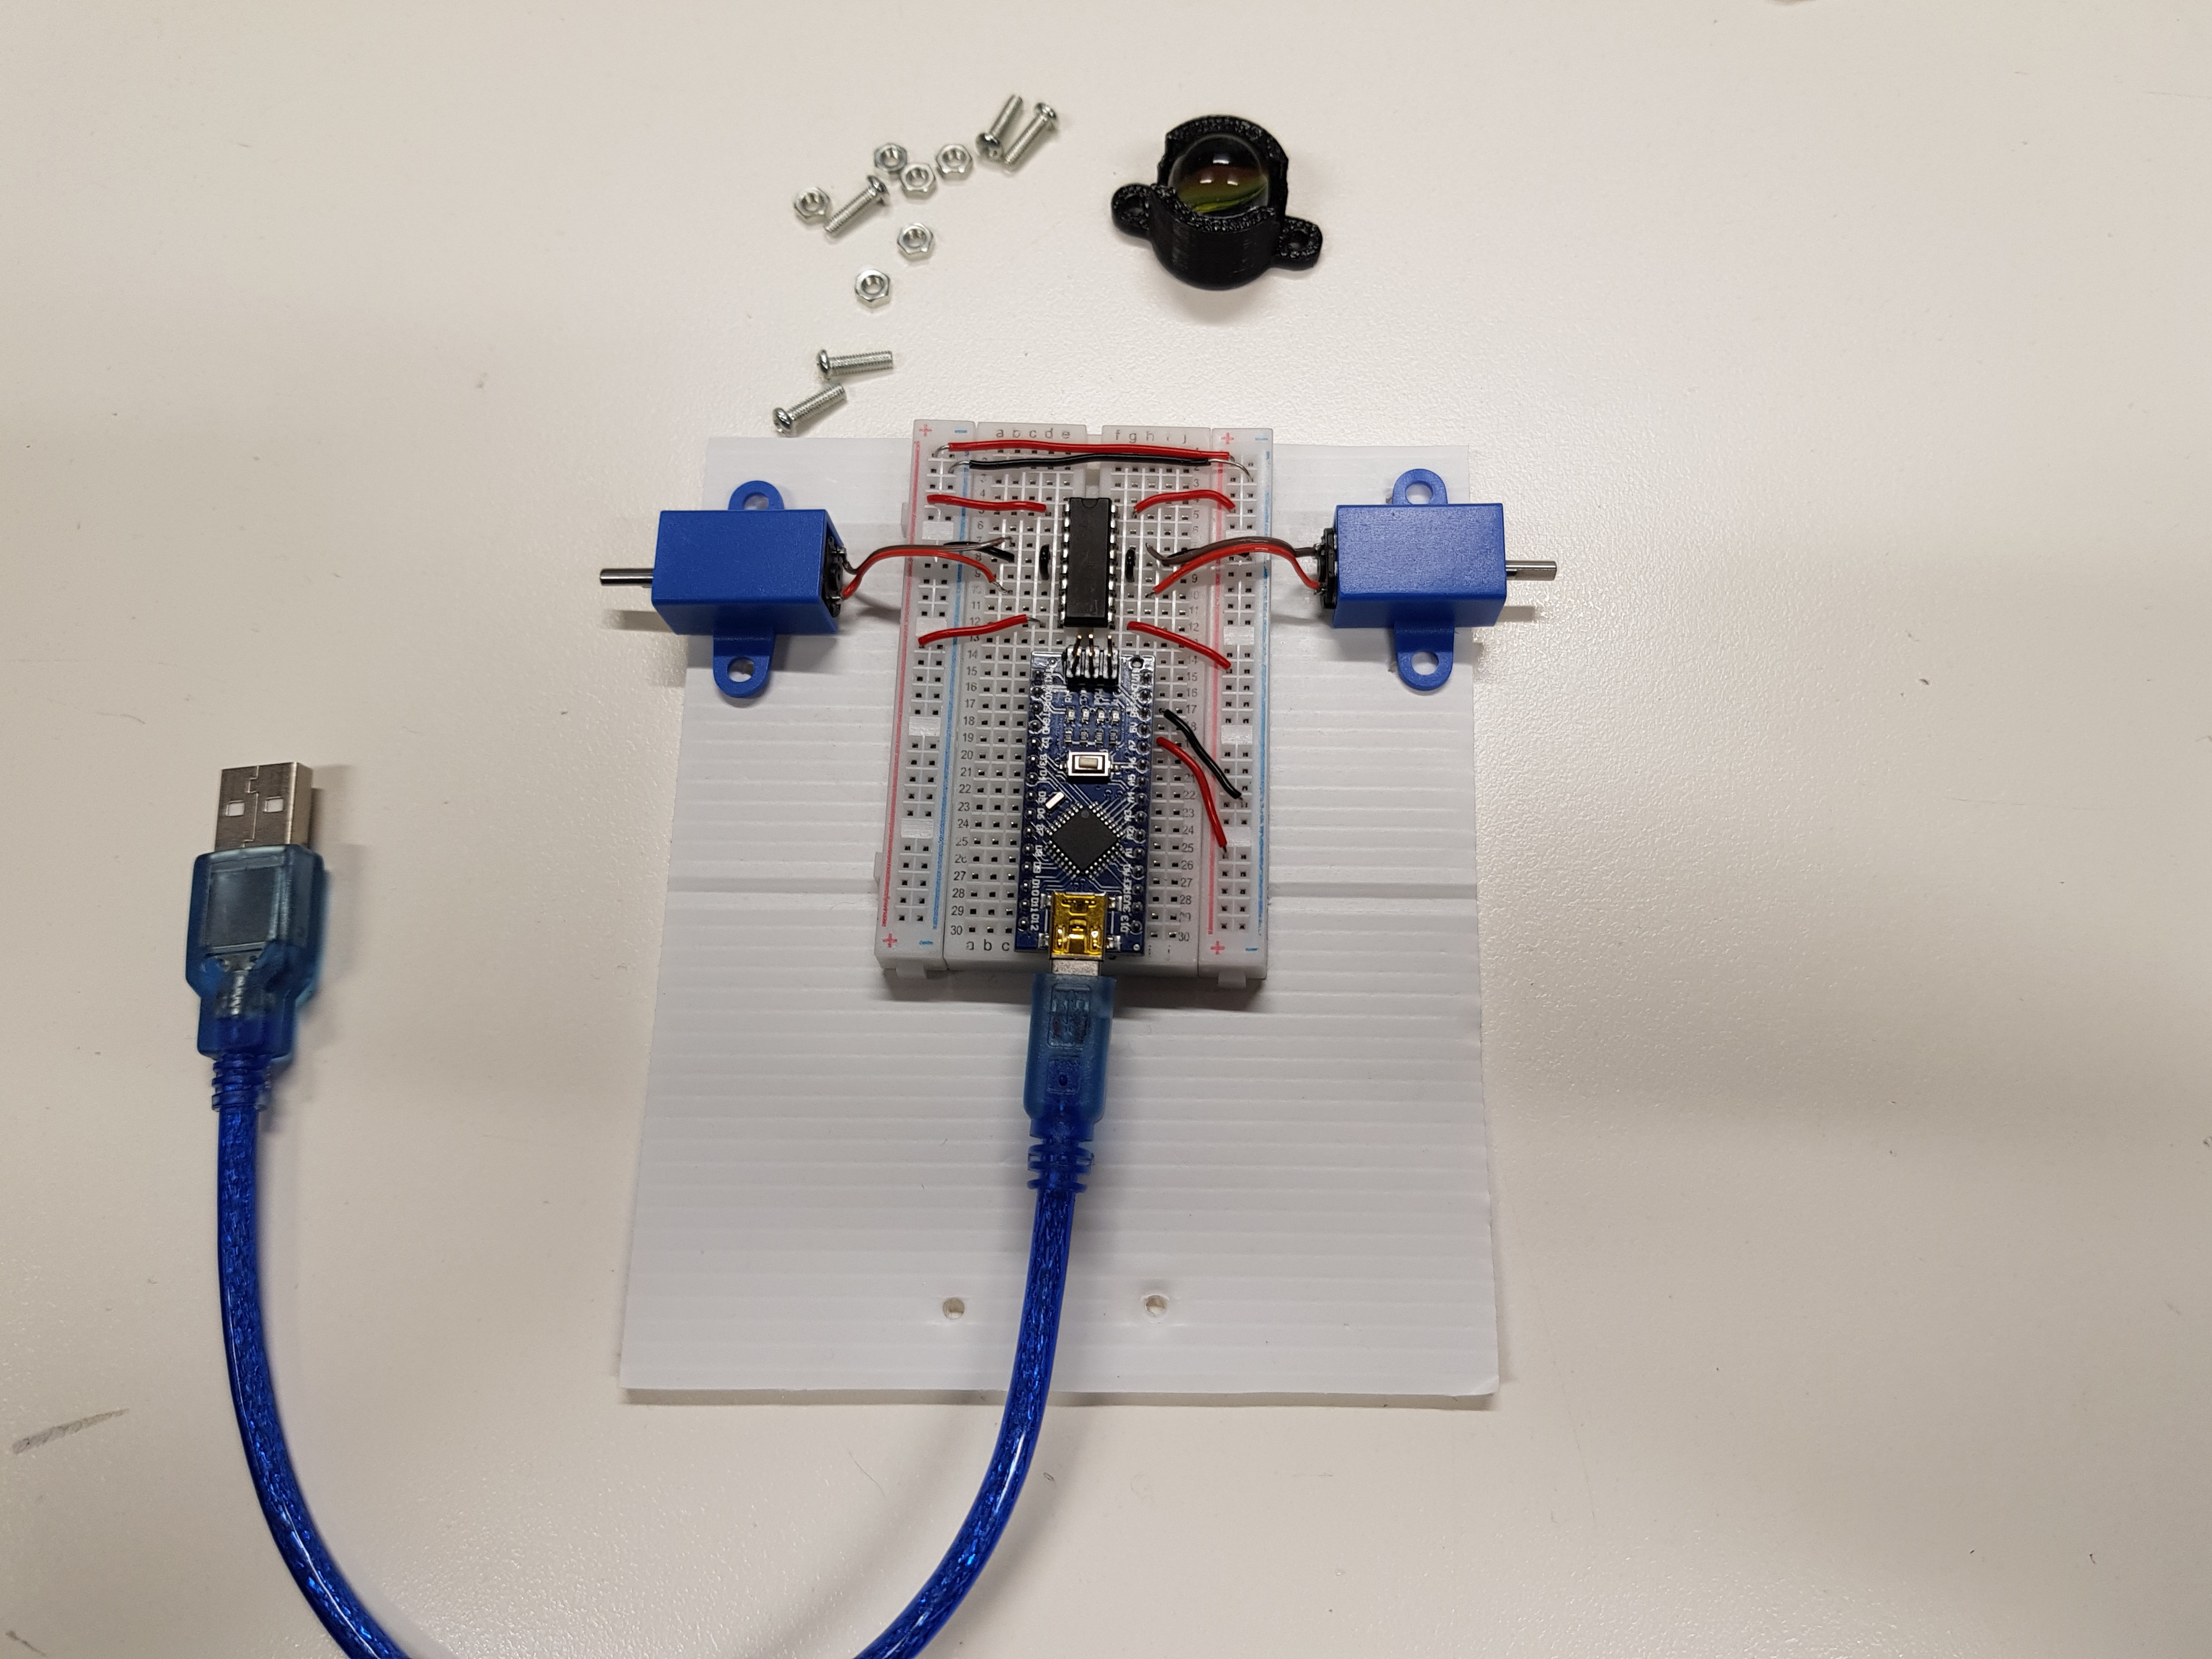
\includegraphics[width=0.6\linewidth]{circuit_base_all_parts_minus_wheels.jpg}
% \end{center}

\begin{center}
    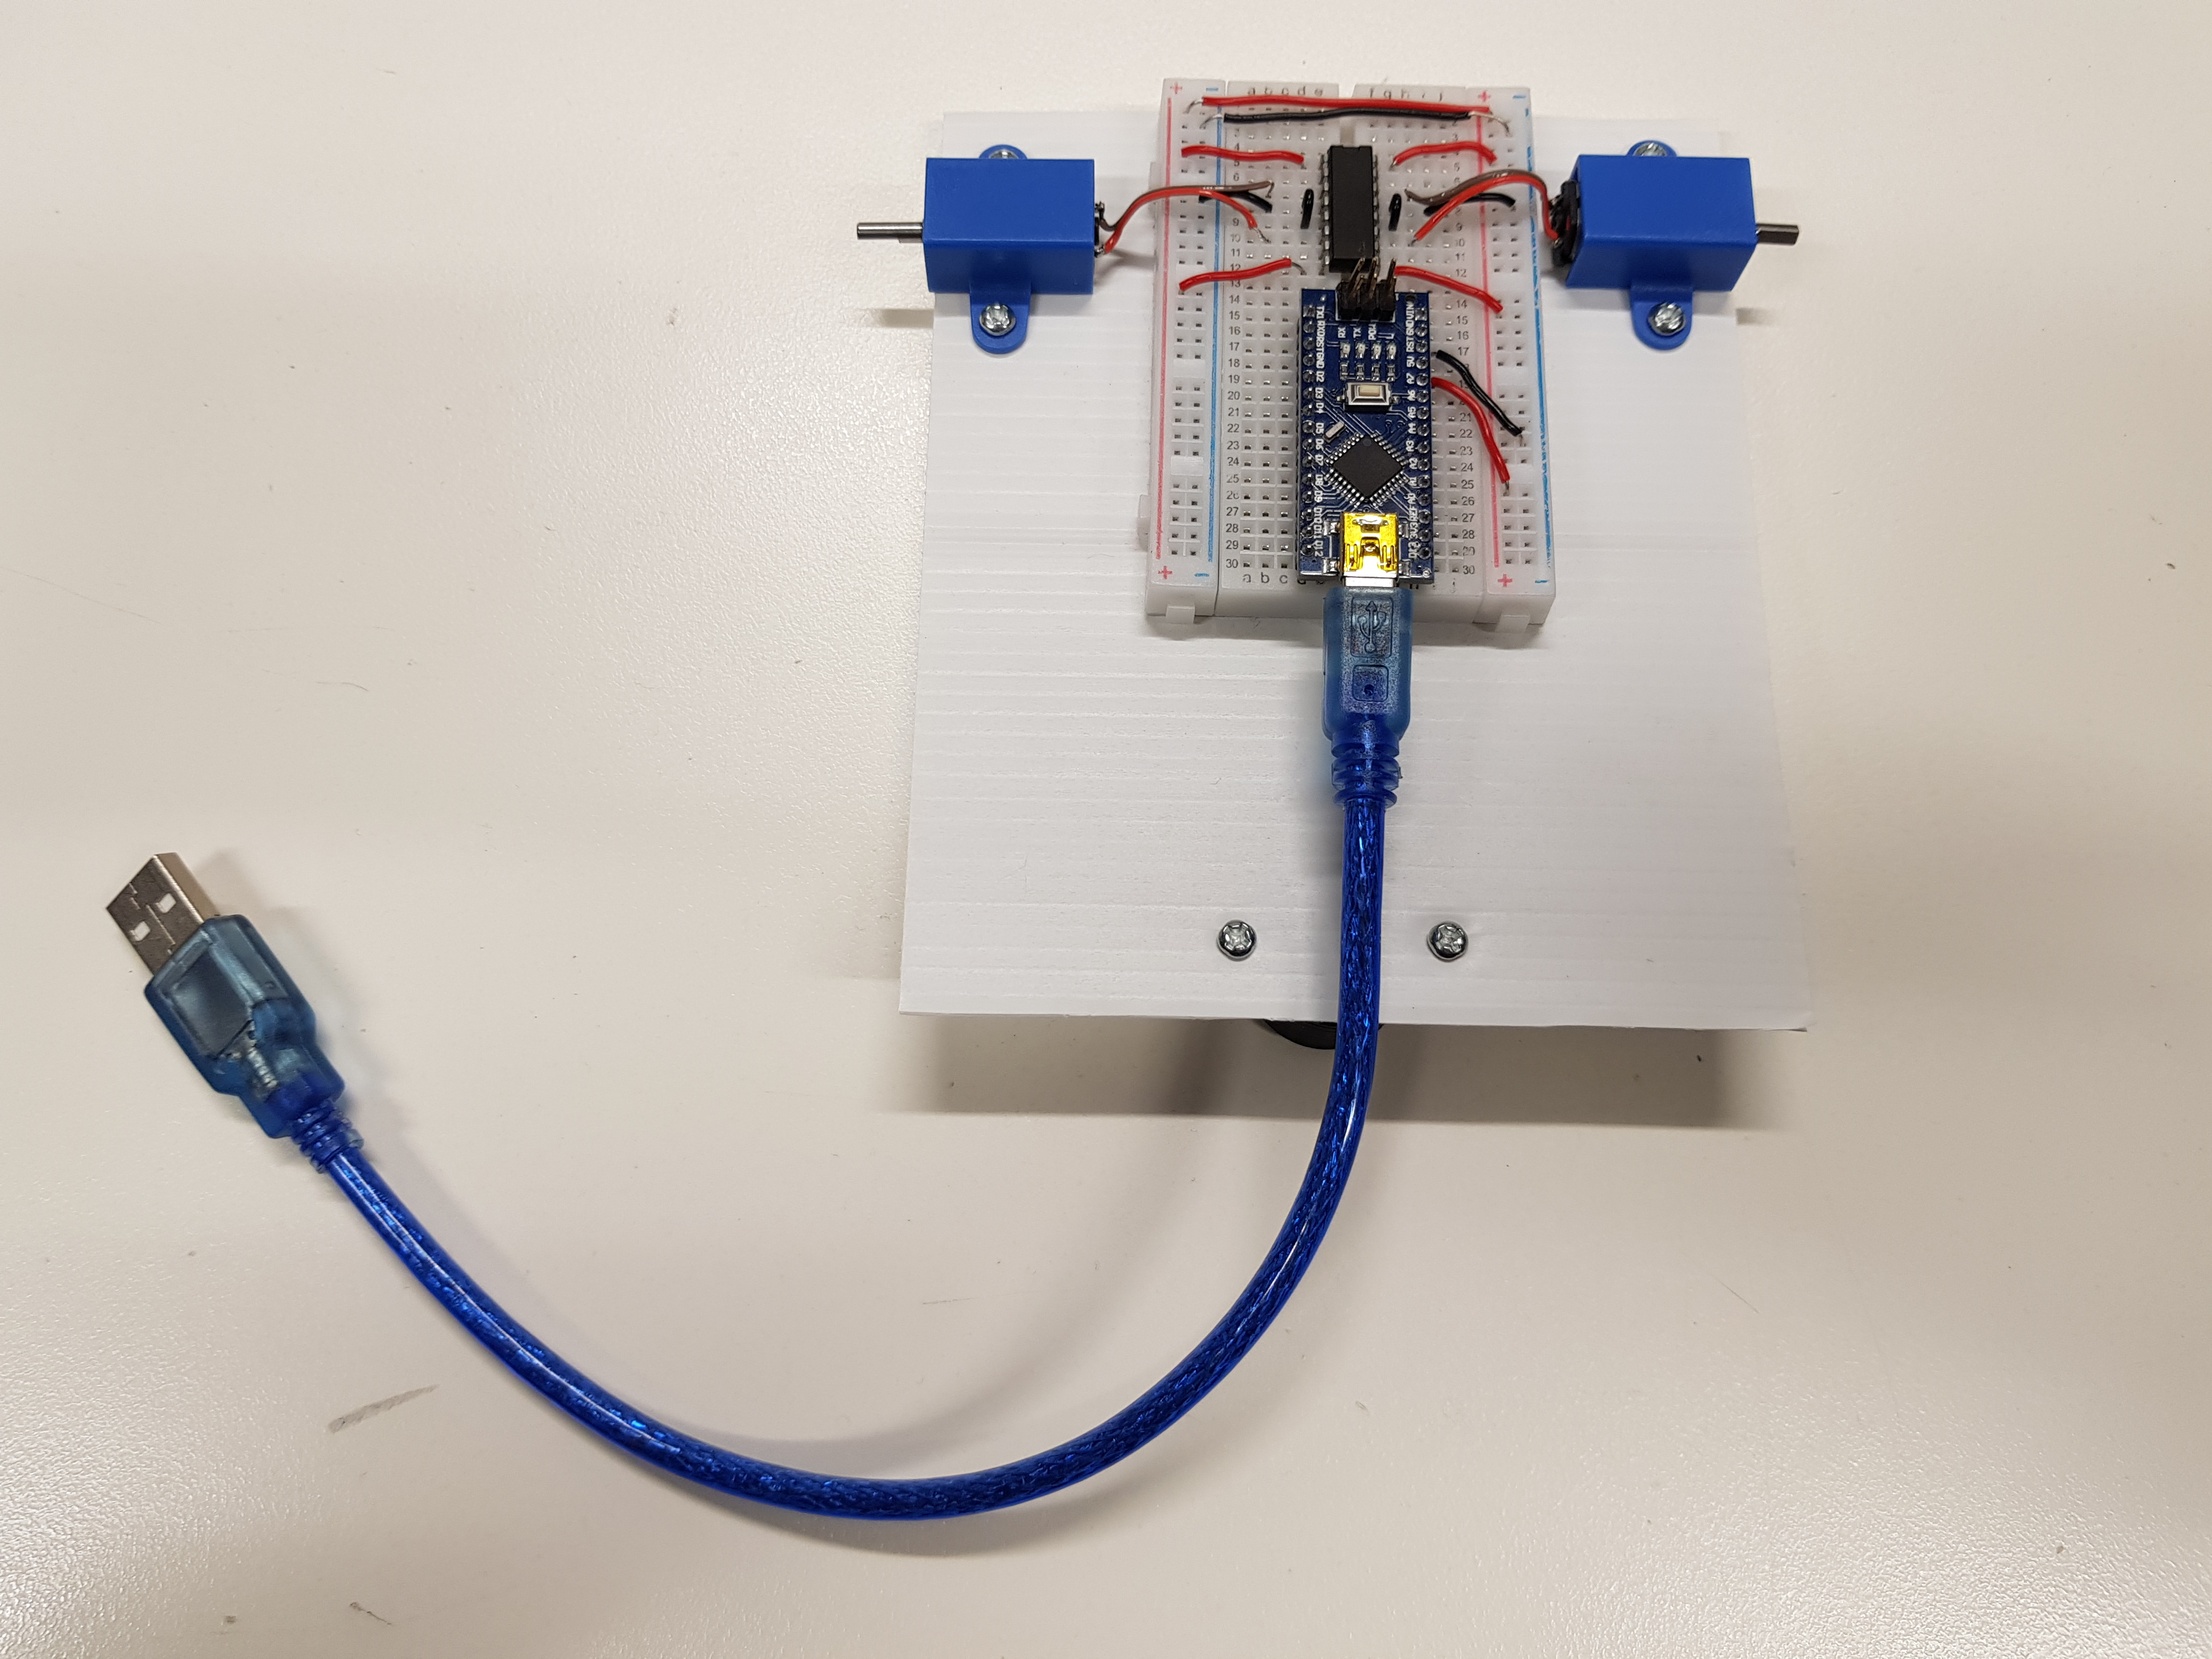
\includegraphics[width=0.6\linewidth]{cover_and_caster_screws.jpg}
\end{center}

Your TinyBot is now fully assembled. (The TinyBot pictured is missing a battery, make sure your TinyBot has a battery)
\begin{center}
    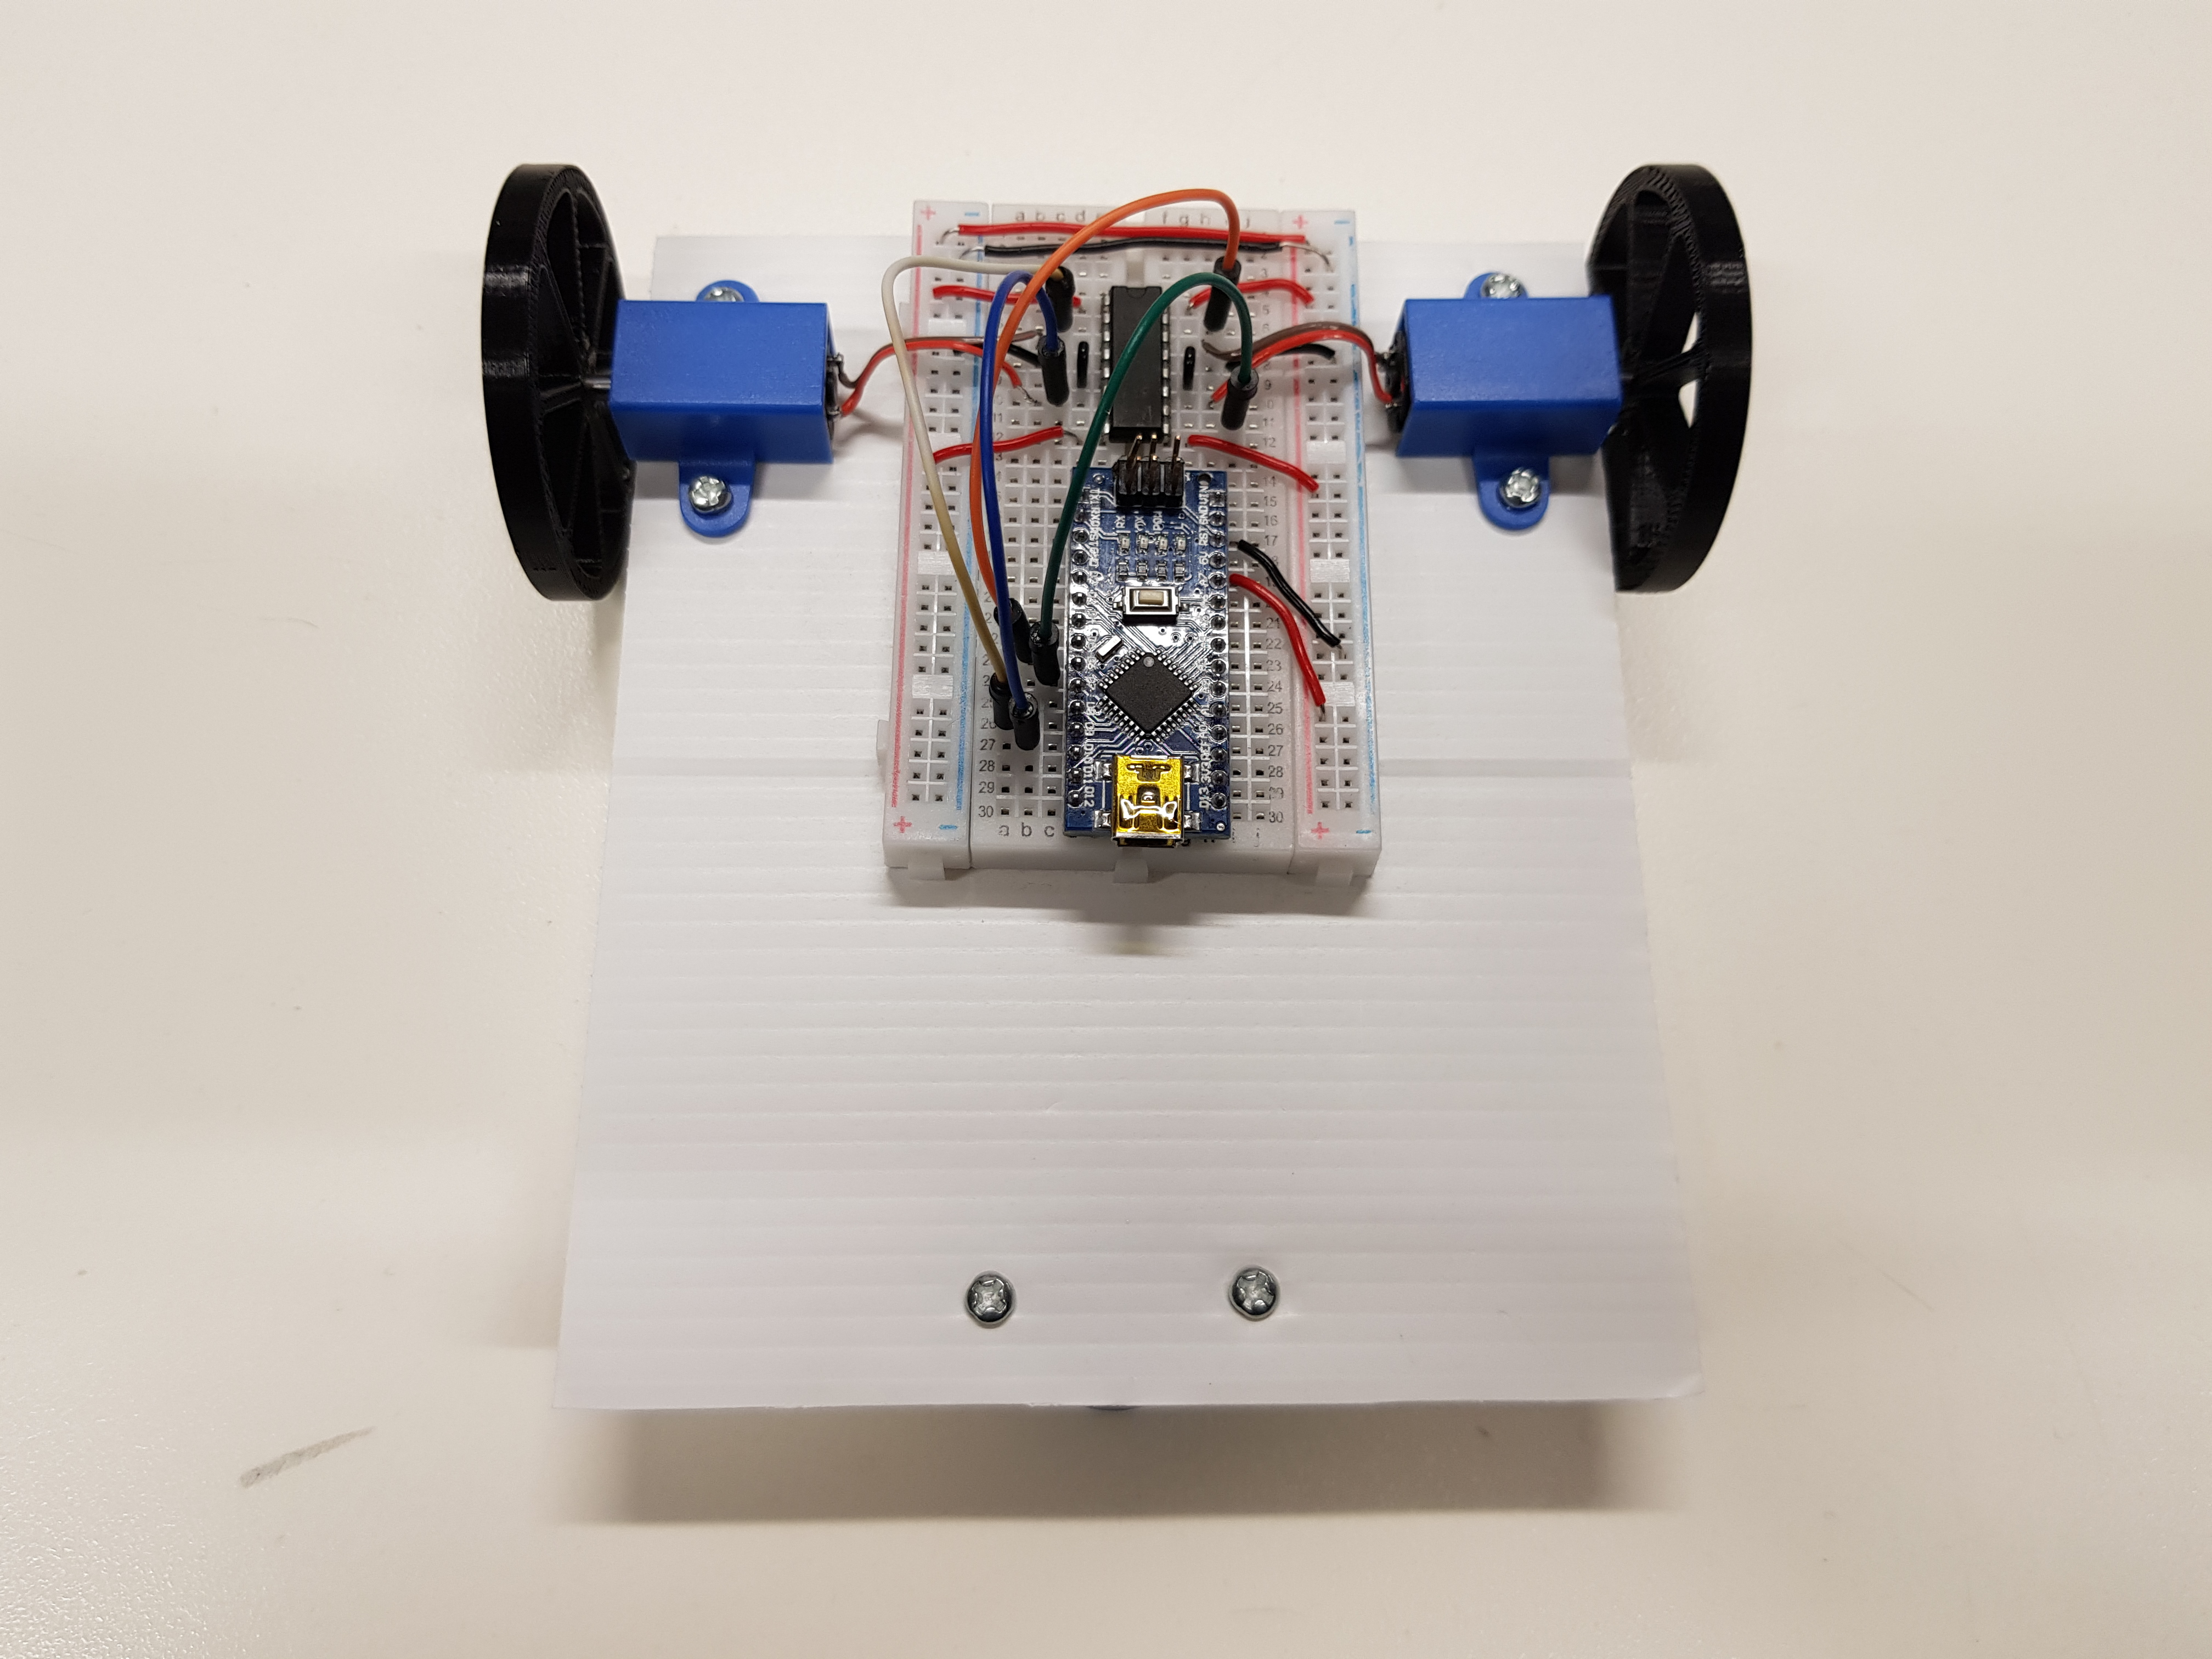
\includegraphics[width=0.6\linewidth]{final_assembled.jpg}
\end{center}

\end{document}